

%----------------------------------------------------------------
% AMS-LaTeX Paper ************************************************
%**** -----------------------------------------------------------
%\documentclass[12pt,twocolumn]{IEEEtran2e}%
%\documentclass[12pt,onecolumn,notitlepage]{report}
\documentclass[12pt,onecolumn,titlepage]{article}
\usepackage{graphicx,epsfig,amsmath,color,listings,tabularx,amsfonts,moreverb}
% ----------------------------------------------------------------
%\vfuzz2pt % Don't report over-full v-boxes if over-edge is small
%\hfuzz2pt % Don't report over-full h-boxes if over-edge is small
% ----------------------------------------------------------------
\newcommand{\code}[1] {\texttt{#1}}
\newcommand{\DB}   {\code{{MOOSDB}}}
\newcommand{\MA}   { \code{{MOOSApp}  }}
\newcommand{\MOOSLIB}   { \code{{MOOSLib}  }}
\newcommand{\New}[1]   {\textbf{\hspace{-15mm} \checkmark \hspace{10mm}#1 }}
\newcommand{\Ignore}[1]   { }
\setlength{\textheight}{230mm} \setlength{\columnsep}{4mm}
\setlength{\textwidth}{157mm} \setlength{\topmargin}{0.25in}
\setlength{\headheight}{0.0in} \setlength{\headsep}{0.0in}
\setlength{\oddsidemargin}{2mm} \setlength{\parskip}{0.03in}
%\pagestyle{empty}

\definecolor{comment}{rgb}{0,0.5,0}
\lstset{
 basicstyle = \small,
 frame = tb,
  language = [Visual]{c++},
  keywordstyle = \color{blue},
  %commentstyle = \color{comment}
  }

\begin{document}


% Produce the title page
\thispagestyle{empty} \vspace{4cm}
\begin{center}
\begin{Huge}
{ MOOS  - Mission Orientated Operating Suite\\ }
\end{Huge}
\vspace{7cm}

%\epsfig{file=moose6.eps,width = 0.2\linewidth} \\
%\epsfig{file=mit_logo_small.eps,width = 0.18\linewidth} \\
\epsfig{file=moose6.eps,width = 0.2\linewidth} \\

\vspace{5cm}
\begin{Large}
{Paul Michael Newman\\ } \vspace{1cm}
%
%
{Department of Ocean Engineering\\ Massachusetts Institute of
Technology\\\vspace{1cm}
Department of Engineering Science\\
Oxford University\\ }
\end{Large}
\vspace{0.5cm} Version 2.1 March 2006
\end{center}



\newpage
\begin{abstract}
This paper is about simple to use, extensible software for mobile
robotic research. It is concerned with a project called MOOS -- an
acronym for Mission Oriented Operating Suite. MOOS is an umbrella
term for a set of libraries and applications designed to
facilitate research in the mobile robotic domain. The spectrum of
functionality provided ranges over  low-level, multi-platform
communications,  dynamic control, high precision navigation and
path planning, concurrent mission task arbitration and execution,
mission logging and playback.

The first part of the paper describes the underlying philosophy of
MOOS and the resulting perceived benefits. The work then moves on
to describe the details of the design and implementations of core
system components. There then follows a set of high level
descriptions of principal mission-oriented MOOS processes.
Collectively these processes constitute a resilient, distributed
and coordinated suite of software suitable for in-the-field
deployment of sub-sea and land research robots.

\end{abstract}


\newpage
\section*{}

\vspace{3cm}
\begin{centering}
\epsfig{file=moose6.eps,width = 0.2\linewidth} \\
\end{centering}
\vspace{3cm}

\section*{Thanks}
First let me thank John for his trust and for believing in and
paying for the MOOS - I've had a ball. The Sea Grant crew made all
the difference, Rob for his advice and un-ending healthy cynicism,
Jim for his tenacity and book of spells , Sam for his skill and
amusing use of the ``pinger'', Joe for great help before, during,
and after trials and Justin for Florida and some great backing. I
very much appreciate their help, enthusiasm and support. Mike
Bosse was a superb client and colleague and always complained
about all the right things - cheers. Richard, thanks for your help
and being a great mate out here. Watch out for flat inert surfaces
- they can hurt a man.

Finally thanks to Sarah. For being great despite too many late
nights at MIT and the occasional ``lost'' weekend, for supplying
cookies and ridiculous MOOS paraphernalia. But most of all for
having made ``Boston'' sane and wonderful. Thank you.

For Version II of this document thanks to Mike Benjamin for excellent critisism
of the software and dedicated use of it. He's also an excellent cookie supplier. Thanks.





\newpage
\tableofcontents

\newpage
\part{Introduction}



\section{Philosophy and Background}
MOOS (pronounced ``moose'')  is an umbrella term applying to a set
of communicating applications. At its most general the ``MOOS''
refers to a suite of libraries and executables designed and proven
to run a field robot in sub-sea and land domains. Included in its
scope are a platform-independent, inter-process communication API,
sensor management such as DVL, LBL and SAS sonar, state of the art
navigation, vehicle dynamic control, concurrent mission task
execution, vehicle safety management, mission logging, mission
replay and reprocessing.

The heart of MOOS, its communications API and Library, was written
over a period of three days in late September 2001. It is the
fourth generation of communications software intended for mobile
robot systems written by the author.  The design of MOOS and the
functionality provided by its communications API was motivated by
experience and observations gained in using and developing several
software suites for mobile robots. In particular it was noted
that:
\begin{itemize}
\item Dependence on a particular operating system is bad news. The
development tools available in one choice may far out-perform
those available in another. Conversely the opposite may be true in
terms of real-time performance and networking. No one choice
satisfies all criteria.
\item Allowing source code dependencies to occur between
different applications can lead to project management problems and
slowed development. As the complexity of the project grows so does
the number of inter-dependencies and time spent coordinating
rebuilds etc.
\item Researchers often require a sense of ownership over an
element of a robotic system. It is desirable to be able to have an
individual write code in his or her own style and in isolation and
yet still have the resulting application interact with any number
of other applications/services running on the vehicle.
\end{itemize}

With these observations in mind the following design goals were
set:
\begin{itemize}
\item Platform independence - Code should run on Linux, NT, and
Win2000.
\item A collection of communicating processes should run the
vehicle - each process encapsulating a specialization or core
functionality.
\item The communications provided to these processes should be
utterly robust and tolerant of repeated stop/start cycling of any
process.
\item Processes should have no shared header file dependencies.
\end{itemize}

\section {Project Management in the Research Domain}
%
It is often the case that executables that need to interact with
each other have a clear 'owner', i.e have been developed on the
whole by a single researcher/engineer. Inevitably then, this work
carries the unique stylistic and architectural finger-prints of
the creator. This development model can be efficient until several
such projects are merged into a monolithic application. It is at
this point that code strain starts to show. Much effort can be
expended in fusing the projects with no overall change in
functionality. MOOS has been designed to allow projects to be
melded without blurring or dissolving process boundaries - the
number of processes remains the same. Instead each process joins a
``community'' of MOOS-enabled applications. Engineers can keep
coding their own application independently of all other source
code. This has ramifications when considering versioning and
source code control. The projects can live completely independent
lives - there is no compiled code dependency between them. A code
change in one domain cannot cause compilation  failures in
another.

\newpage
\part{Foundations}
\section{Overview}
It is useful to provide a brief description of a typical MOOS
driven system to provide a compelling motivation for the rest of
this document.

Consider the case of an single AUV (autonomous underwater vehicle)
operating within an LBL (long base-line) acoustic array
\footnote{MOOS can and has been equally well applied to land
robots however the AUV example is pretty interesting}. MOOS
provides all the software components and communications required
manage sensors, navigate, control actuators, plan trajectories,
monitor safety , log performance and both manual and automatic
control.
\begin{figure}[h!]\label{fig:Example}
\centering \epsfig{figure = Example.eps,width = 0.8\linewidth}
\caption{A complete MOOS configuration for AUV deployment. Taken
from the ``GOATS 2002'' experiment, Italy 2002}
\end{figure}
Figure \ref{fig:Example} shows a typical consortium of processes
used on a typical AUV research mission. In fact this setup was
used during the ``GOATS 2002'' experiment in Italy 2002. The AUV
was carrying a synthetic aperture sonar managed by a separate PC
in a payload section. MOOS enabled seem-less integration of this
payload with the processes running on the main vehicle computer
while providing real-time navigation and control of the vehicle
using a multitude of sensors. The details of these processes and
more importantly the underlying infrastructure will be discussed
in future sections of this document. At this juncture the most
important message to take home is that MOOS is a designed to
provide:
\begin{enumerate}
\item A standardized, multi-platform way for processes to share information
\item A set of key processes that fulfill ubiquitous roles in
mobile robotics
\end{enumerate}




\section{Topology}
MOOS has a star-like topology. Each application within a MOOS
community ( a \MA) has a connection to a single ``MOOS Database''
(called \DB) that lies at the heart of the software suite. All
communication happens via this central ``server'' application. The
network has the following properties:
\begin{itemize}
\item No Peer to Peer communication.
\item All communication  between the client and server is instigated by the
client. (ie the \DB {\textbf{never}} makes a unsolicited attempt
to contact a \MA.)
\item Each client has a unique name.
\item A given client need have no knowledge of what other clients exist.
\item A client has no way of transmitting data to a given client -
it can only be sent to  the \DB.
\item The network can be distributed over any number of machines
running any combination of supported operating systems.
\end{itemize}
This centralized topology is obviously vulnerable to
``bottle-necking'' at the server regardless of how well written
the server is. However the advantages of such a design are perhaps
greater than its disadvantages. Firstly the network remains simple
regardless of the number of participating clients. The server has
complete knowledge of all active connections and can take
responsibility for the allocation of communication resources. The
clients operate independently  with inter-connections. This
prevents rogue clients (badly written or hung) from directly
interfering with other clients.

\begin{figure}[ht!]
\centering  \epsfig{figure=Topology.eps,width=0.4\linewidth}
\caption{MOOS binds applications into a network with a star-shaped
topology. Each client has a single communications channel to a
server (\DB).} \label{fig:Topology}
\end{figure}

\section{MOOS Communities (and multiples
of)}\label{sec:Communities}

\New{} Post 2002 releases of MOOS have included explicit support
for multiple communities. The idea is that is is sometimes
advantageous to have groups of processes (bound together by mutual
connection to a MOOSDB hub) communicating with each other. To this
end, MOOSMsg's have been extended to included a ``Source
Community'' field which names the community from whence the
message came.

Under the ``one mission one mission file'' paradigm process
running on in community reads from the same mission file (see
section \ref{sec:ConfigFile}. The community name is specified by
the line \code{Community = <Name> } at the top of the mission
file. \footnote{Perhaps near the \code{ServerPort=} and
\code{ServerHost=} global definitions.}

The question remains --- how does this information get used? Well,
when the MOOSDB serving each community starts up (see Section
\ref{sec:DB}) the community name will be read and all messages
sent from the DB will be tagged with this community name (see
Section \ref{sec:Content}. However this tagging only happens if
the data content originated from the \DB's own local community
--- if it did not (i.e. it came from another community) then the
community name of the orginating community is preserved. To
understand how data from an external community could appear in one
particular \DB see section \ref{Sec:pMOOSBridge}.

\section{Message Content}\label{sec:Content}
The communications API in MOOS allows data to be transmitted
between \DB and a client. The meaning of that data is dependent on
the role of the client. However the form of that data is
constrained by MOOS. Somewhat unusually MOOS only allows for data
to be sent in string or double form. Data is packed into messages
(CMOOSMsg class) which contains other salient information shown in
Table \ref{tab:MOOSMsg}.
\begin{table*}
\centering
\begin{tabular}{l|l}\hline
  % after \\: \hline or \cline{col1-col2} \cline{col3-col4} ...
  {\textbf{Variable}} & {\textbf{Meaning}} \\ \hline
  Name  & The name of the data \\
  String Val & Data in string format \\
  Double Val & Numeric double float data \\
  Source & Name of client that sent this data to the \DB \\
  Time & Time at which the data was written \\
  Data Type & Type of data (STRING or DOUBLE)  \\
  Message Type & Type of Message (usually NOTIFICATION) \\
\New{Source Community} & The community to which the source process
belongs---see Sec \ref{sec:Communities}\\\hline
\end{tabular}\vspace{7mm}
  \caption{Contents of MOOS Message}\label{tab:MOOSMsg}
\end{table*}
The fact that data is commonly sent in string format is often seen
as a strange and inefficient aspect of MOOS. For example the
string \verb"Type=EST,Name=AUV,Pos=[3x1]{3.4,6.3,-0.23}" might
describe the position estimate of a vehicle called ``AUV'' as a
3x1 column vector\footnote{Typically string data in MOOS is a
concatenation of comma separated "name = value" pairs.}. It is
true that using custom binary data formats does decrease the
number of bytes sent. However binary data is unreadable to humans
and requires structure declarations to decode it and header file
dependencies are to be avoided where possible. The communications
efficiency argument is not as compelling as one may initially
think. The CPU cost invoked in sending a TCP/IP packet is largely
independent of size up to about one thousand bytes. So it is as
costly to send two bytes as it is one thousand. In this light
there is basically no penalty in using strings. There is however a
additional cost incurred in parsing string data which is far in
excess of that incurred when simply casting binary data.
Irrespective of this, experience has shown that the benefits of
using strings far outweighs the difficulties. In particular:
\begin{itemize}
\item Strings are human readable - debugging is trivial especially
using a tool like MOOSScope. (see Section \ref{sec:MOOSScope})
\item All data becomes the same type
\item Logging files are human readable (they can be compressed for
storage).
\item Replaying a log file is simply a case of reading strings from
a file and ``throwing'' them back at the \DB in time order.
\item The contents and internal order of strings transmitted by an application can be changed
without the need to recompile consumers (subscribers to that data)
- users simply would not understand new data fields but they would
not crash.
\end{itemize}
Of course, scalar data need not be transmitted in string format -
for example the depth of a sub-sea vehicle. In this case the data
would be sent while setting the data type to  \verb"MOOS_DOUBLE"
and writing the numeric value in the double data field of the
message.

\section{Threading and Process Models}
The choice of processes over threads was made on two counts,
firstly that of stability - a rogue process cannot corrupt the
program/data space of another process (in a sane OS that is).
Secondly on the basis of swift and pain-free development by
several programmers with diverse backgrounds. Building a single
monolithic executable by several people requires, at a minimum,
adherence to programming guidelines and styles that may not be
native to all those included - especially in an academic
environment. The use of small-footprint, independent processes
implies developers can use whatever means they see fit to
accomplish the job. Linking with the communications library
integrates them seamlessly with all other processes but denies a
process the means of interfering with others.



\section{Communications Mechanics}
%%%%%%%%%%%%%%%% FIGURE %%%%%%%%%%%%%%%%%%%%%%%%%%%%%%
\begin{figure*}[ht!]
\centering \epsfig{figure = Comms.eps,width = 1.0\linewidth}
\caption{The mechanics of the client server interaction in MOOS.
The user code calls the \code{Notify} method to transmit data.
This method simply adds a message to the ``outbox''. Some time
later (1) the communications thread calls into the database. When
the database is not busy it accepts the client's call (2). The
client then packs the entire outbox into a single large
transmission which is sent to and read by the server (3). The
server unpacks the packet into its constituent messages and place
copies (according to subscriptions and timing ) in the mailboxes
of other connected clients. The server then compresses the mailbox
of the current client into a packet and sends it back to the
client (4). At this point the transaction is then complete and the
server terminates the conversation and looks to begin the same
process with a different client. Upon receiving the reply packet
the client communications thread unpacks it and places the
resulting messages in the ``inbox'' of the client. The user code
can retrieve this list of messages at {\it{any time}} by calling
the \code{Fetch} method.}
\end{figure*}

Each client has a connection to the DB. This connection is made on
the client side by instantiating a class provided in the core
\code{MOOSLIB} library called \code{CMOOSCommClient}. This class
manages a private thread that coordinates the communication with
the \DB. The \code{CMOOSCommClient} object completely hides the
intricacies and timings of the communications from the rest of the
application and provides a small, well defined set of methods to
handle data transfer. Using the \code{CMOOSCommClient} each
application can:
\begin{enumerate}
\item Publish data - issue a notification on named data.
\item Register for notifications on named data.
\item Collect notifications on named  data.
\end{enumerate}

\subsection{Publishing Data - notification} Assume as a result of
 some computation or input, a process \code{A} has a result that
is likely to be of use other undisclosed (remember MOOS
applications do not know about each other) processes \code{B} and
\code{C} - for example a position estimate. The simplest way in
which \code{A} can transmit its new data is to simply call the
\code{Notify} method on its local \code{CMOOSCommClient} object
specifying the data, its name and the time at which it is valid.
Behind the scenes this method then creates a suitable
\code{CMOOSMsg} filling in the relevant fields. The action of
publishing data in this way should be viewed as a
{\emph{notification}} on a named data variable. Crucially this
does not imply a change in the {\emph{value}} - the outcome of the
computations resulting in the need to publish data may remain not
change . For example two sequential estimates of location of a
vehicle may remain numerically the same but the {\it{time}} at
which they are valid changes - this constitutes a data
notification.

As far as the application-specific code in \code{A} is concerned
the invocation of the \code{Notify} method results in the data
being sent to the \DB. What is really happening however is that
the \code{CMOOSCommClient} object is placing the data in an
``outbox''  of \code{CMOOSMsg}s that need to be sent to the \DB at
the next available opportunity. The next obvious question is
``when does the  data reach the \DB?''. The \code{CMOOSCommClient}
object thread has a ``Comms Tick'' - essentially a timer that
contacts the \DB at a configurable rate (typically 10Hz but up to
50Hz ). All the messages in the outbox are packed into a single
packet or ``super message'' called a \code{CMOOSPkt}. Eventually
the \DB will accept the incoming call from the client \code{A} and
receive the packet. At this point the data flow is reversed and
the \DB replies with another \code{CMOOSPkt} containing
notifications (issued by other processes like \code{B} and
\code{C}) that are relevant to  \code{A}. How a process declares
what constitutes a relevant notification is discussed in section
\ref{sec:Registration}. If at the time the thread calls into the
\DB the outbox is empty (i.e there is nothing to notify) a NULL
message is created and sent. Similarly the \DB my reply with a
\code{CMOOSPkt} containing only a NULL message if  nothing of
interest to the client has happened since its last call in. This
policy preserves the strict symmetry of ``one packet sent, one
packet received'' for all occasions.


\subsection{Registration}\label{sec:Registration} Assume that a
list of names of data published has been provided by the author of
a particular MOOS application. For example, a application that
interfaces to a GPS sensor may publish data called \code{GPS\_X}
and \code{GPS\_Y}. A different application may register its
interest in this data by {\it{subscribing }} or {\it{registering}}
for it. An application can register for  notifications using a
single method \code{Register} specifying both the name of the data
and the maximum rate at which the client would like to be informed
that the data has been changed. The latter parameter is specified
in terms of the minimum possible time between notifications for a
named variable. For example setting it to zero would result in the
client receiving in the \code{CMOOSPkt} (that is the \DB's reply)
a collection of messages describing each and every change
notification issued on that variable.

\subsection{Collecting Notifications}\label{sec:CollectingNotifications}
At any time the owner of a \code{CMOOSCommClient} object can
enquire whether it has received any new notifications from the \DB
by invoking the \code{Fetch} method. The function fills in a list
of notification \code{CMOOSMsg}s describing what has changed, what
client made the change, when it was done and what the data type is
(see table \ref{tab:MOOSMsg} in section \ref{sec:Content}). Note
that a single call to \code{Fetch} may result in being presented
with several notifications corresponding to the same named data.
This implies that several changes were made to the data since the
last client-server conversation. However, the time difference
between these similar messages will never be less than that
specified in the \code{Register} function described in section
\ref{sec:Registration}.


\section{The MOOSDB}\label{sec:DB}
The \DB is the heart of the system. It serves as the hub through
which all communication occurs. It is tempting to think of the \DB
as simply a blackboard - an entity which stores the current state
(represented by values of named variables) of the system.
Typically a blackboard allows clients shared access to a
centralized repository of information. Although the \DB does
maintain the most recently set value of all variables and in that
way is similar to a blackboard, the way in which data is retrieved
is very different. The \DB records, on  behalf of its connected
clients, the {\it{history}} of changes to data. Assume a client
\code{A} has subscribed to variables called \code{p} and \code{q}
with a minimum notification period of $\tau_{p}$ and  $\tau_{q}$
seconds respectively. The time is now $t$ and the last call-in was
at time $t'$,$\Delta = t-t'$ seconds ago. When \code{A} calls in,
it is not simply presented with the most recent values of \code{p}
and \code{q} but rather all the {\it{changes}} that have occurred
to them between $t'$ and $t'$. Imagine that some other process
\code{B} is publishing changes (value and/or time-stamp) to $p$
and $q$ every $\tau_B$ seconds. The call in will result in $n_p$
and $n_q$ notification messages being returned to the client where
\begin{align*}
n_p &= \begin{cases}
    floor(\frac{\Delta}{\tau_{p}}) & \text{$\tau_{p} \geq \tau_B$}, \\
    floor(\frac{\Delta}{\tau_{B}}) & \text{otherwise}.
  \end{cases}\\
n_q &= \begin{cases}
    floor(\frac{\Delta}{\tau_{q}}) & \text{$\tau_{q} \geq \tau_B$}, \\
    floor(\frac{\Delta}{\tau_{B}}) & \text{otherwise}.
  \end{cases}
\end{align*}

If no clients have issued relevant notifications since $t'$ then
there will be no notification messages stored at the \DB for
collection by the client. The only exception to this rule is the
first time a client calls in after registering for a notification
on a variable. In this case the value of the variable is returned
in a notification message with a time-stamp specifying when the
data was last set.

\newpage
\part{Using The MOOS -- Libraries and Classes}


The combination of the \DB and the two libraries \code{MOOSLib}
and \code{MOOSGenLib} are all that is needed to build a MOOS
community. The role and operation of the \DB has already been
discussed in section \ref{sec:DB}. The contents and utilities
provided by the libraries are now described.

\section{MOOSLib}
The primary role of \code{MOOSLib} is to contain all the
communications components used both by the \DB itself and
\code{CMOOSCommClient} objects owned and used by client
applications.
\subsection{\code{CMOOSApp}}\label{sec:CMOOSApp}
 Perhaps the most important class exposed from the library is \code{CMOOSApp}. This class should be
used as  a base class for all MOOS applications. It provides along
with other things:
\begin{itemize}
\item Management and configurations of a \code{CMOOSCommClient} object
\item Tools for reading configuration parameters (using a file
reading tool exported from \code{MOOSGenLib}).
\item Timing control of the main thread of the application and an
additional communications thread.
\item Virtual functions that can be overloaded to perform specific
actions when:
\begin{enumerate}
\item New mail (notifications) arrives
\item The default work of the application should occur
\item The client connects to the \DB
\item The client disconnects from the server
\item The application is about to start
\end{enumerate}
\end{itemize}
Appendix A gives example code of a skeleton MOOS application using
the functionality provided by deriving from \code{CMOOSApp}.
Indeed this code could be used as the template from which to start
building all new MOOS applications. The timing of the application
is determined by two timer frequencies \code{AppTick} and
\code{CommsTick} which are set in the process configuration file
(see section \ref{sec:ConfigFile}). The \code{CMOOSApp} base class
does its best to call the virtual \code{Iterate} method at the
frequency specified by \code{AppTick}. It is within this method
that the bulk of the work of the application should be undertaken
- for example processing data or executing control loops. Just
before \code{Iterate} is called the \code{CMOOSApp} base class
calls \code{Fetch} (see section \ref{sec:CollectingNotifications}
on its \code{CMOOSCommClient}. If mail is present then the virtual
function \code{OnNewMail} is called. Here an overloaded version is
passed a list of \code{CMOOSMsg}s which can contains the relevant
notifications from the \DB and which can be acted upon as the
application sees fit. Only messages corresponding to variables
that have been registered for will be present. Typically an
application registers its interest in named data by calling
\code{CMOOSCommClient::Register()} during the virtual callback
\code{OnConnectToServer()}. This guarantees that the server has
been found, successfully connected to and subsequently any
registrations shall be successful. It should be noted that
attempting to register outside of this function (for example in
the overloaded \code{OnStartUp} method) may fail because the
communications thread with \code{CMOOSCommClient} has not yet
established a connection with the \DB.

\subsection{\code{CMOOSInstrument}} The class
\code{CMOOSInstrument} is another important base class. It is
intended to simplify the writing of applications interacting with
hardware via a single serial port. The class extends
\code{CMOOSApp} with utilities to manage and set up a
platform-independent serial port\footnote{The serial port classes
live in \code{MOOSGenLib} - see section \ref{sec:GenLib}.}. The
serial port can be configured to be asynchronous and receive
unsolicited streaming data or to be synchronous and perform
blocking read and writes. The choice  depends on the device the
application is intended to communicate with.

\section{MOOSGenLib}\label{sec:GenLib} The library
\code{MOOSGenLib} is a tool chest. It contains utilities and
classes used throughout MOOS. In particular it provides:
\begin{itemize}
\item Platform-independent serial ports (asynchronous and
synchronous).
\item Thread safe configuration reading tool
-- \code{CMOOSMissionFileReader}.
\item String manipulation/parsing tools.
\item Geodesy tools.
\item debug statement tools - MOOS equivalent of \code{printf}.
\end{itemize}
Of these assets the configuration file reader in particular
warrants more discussion.

\subsection{Configuration Files *.moos}\label{sec:ConfigFile}
Every MOOS process can read configuration parameters from a
``Mission file'' which by convention has a ``.moos'' extension.
For example the default mission file mentioned in the example code
given in Appendix A is {\it{Mission.moos}}. Traditionally MOOS
processes share  the same mission file to the maximum extent
possible. For example it is usual for there to be one common
mission file for all MOOS processes running on a given machine.
Every MOOS process has information contained in a configuration
block within a *.moos file. The block begins with the statement
\begin{center}
\code{ProcessConfig} = \code{ProcessName}
\end{center}
where {\code{ProcessName}} is the unique name the application will
use when connecting to the \DB. The configuration block is
delimited by braces. Within the braces there is a collection of
parameter statements - one per line.

Each statement is written as
\begin{center}
\code{ParameterName = Value}
\end{center}
where \code{Value} can be any string or numeric value. Typically
the format of the value string is a comma separated list of
strings or numbers. However some applications may require more
complicated syntax using a combination of delimiters other than
simple commas. Of course, the details of these settings is part of
the application documentation. Examples can be found on the MOOS
website ({\it{http://oceanai.mit.edu/pnewman}}). All applications
deriving from \code{CMOOSApp} and \code{CMOOSInstrument} inherit
several important configuration options. For example,
\code{CommTick} and \code{AppTick} (see section
\ref{sec:CMOOSApp}. The documentation on the MOOS webpage gives
details of these common parameters.

\begin{figure}\label{fig:ProcConfig}
\caption{A typical configuration block for a MOOS application. A
process called ``iDepth'' will search a mission file until a block
like this is found. It will then parse our configuration
parameters.}
\begin{lstlisting}[language = {matlab}]{}
/////////////////////////////
// depth sensor configuration
ProcessConfig = iDepth
{
    AppTick = 8
    CommsTick   = 4
    Port        = com1
    BaudRate    = 9600
    Streaming   = false
    Type        = ParaSci
    Resolution  = 0.1
}
\end{lstlisting}
\end{figure}
Figure \ref{fig:ProcConfig} gives an example of a typical
configuration block, in this case for a depth sensor. The
parameters \code{Type} and \code{Resolution} are specific to the
class defining the methods of a ``DepthSensor''. All the other
parameters are handled by its base classes (\code{CMOOSInstrument}
and \code{CMOOSApp}).

\subsection{Utility Functions}
\code{MOOSGenLib} contains a host of utility functions that are
described below. These functions are ubiquitous within MOOS and
should not be substituted with local version producing the same
functionality. The reason is the innards if these functions may be
built to accommodate subtleties in MOOS. A good example is that of
\code{MOOSTime} which returns the current process time
{\em{corrected}} by a constant term setup by the MOOS
communications when the server is contacted.

\begin{description}
  % after \\ : \hline or \cline{col1-col2} \cline{col3-col4} ...
%
\item[\code{MOOSFormat}]  The MOOS version of \code{sprintf}. It
  returns a formatted \code{std::string}  object.
%
\item[\code{MOOSTrace}]  The MOOS equivalent of \code{printf} printing
 a formatted string to the console. When run under win32 the
  function also writes to a debugger window if applicable. Note
  that   \code{MOOSTrace} does not use \code{cout} because on some
  Linux releases this is not thread safe.
%
\item[\code{MOOSChomp}]  A massively useful, simple string parsing
  function.   \code{MOOSChomp} is passed a string, S, to act on and a
  delimiter string, D, as parameters. It returns the substring
  occurring before D in S and removes everything up to
  the end of the D from the S. For example if S = ``X = 4, Y = 9''
  and D =``,'' then calling \code{MOOSChomp(S,D)} would return ``X =
  4'' and S would now be ``Y=9''.

\item[\code{MOOSTime}]  Returns the current time in decimal seconds (a
  double) for the current process. All connected processes will
  show the same time {\em{even}} if their respective machine clocks
  differ. This is achieved by deducing a client correction during initial handshaking with the
  \DB.
%

\item[\code{MOOSGetTimeStampString}] returns a time/date string formatted
in the MOOS convention - useful for naming temporary local files
for development purposes etc.
%
\item[\code{MOOS\_ANGLE\_WRAP}] Wraps all angles (in radians) to be
with $\pm \pi$ - forgetting to wrap angles can cause woe.
%
\item[\code{MOOSPause}] Pauses the current thread (not process) for
a specified number of milliseconds.
\item[\New{\code{MOOSGetValFromString}}]. Extracts named token=val
pairs from a string. For example: \newline
\code{name=AUV1,pose=[3x1]\{2,3,4\}}\\
Note the formatting of the vector - matrices can also be parsed in
this way. The function fills in a reference to
\code{std::vector<double>} and references to the rows and columns
that have been squeezed into this flatend form.
\end{description}


\subsection{Serial Ports}
The \code{CMOOSInstrument} class extends the \code{CMOOSApp} class
to offer non-blocking serial port functionality. The serial port
operations can be one of two modes - synchronous and asynchronous.

\begin{description}
\item[Synchronous] This mode is designed to be applied to
instruments that are synchronous - that is they only talk when
asked to. When in this mode the serial port owner is  responsible
for sending commands and listening (with a timeout) for replies as
required. It is the simplest mode and commonly employed.
\item[Asynchronous / Streaming] This mode is designed for use with instruments
that issue a stream of unsolicited transmissions. In this case the
serial port class manages a listen thread that parses incoming
bytes into a  series of telegrams, which are stored  along with a
time stamp in a list. The characters/bytes that delimit an end of
telegram in the input stream can be changed on the fly. At any
time the serial port user can query the store of telegrams to
retrieve a message or perhaps purge the list of its contents.
\end{description}

\newpage
\part{MOOS Conventions}

\section{Coordinate Conventions}
MOOS processes communicate using a defined coordinate system
illustrated in figure \ref{fig:coordinates}. The salient points to
note about this system are:
\begin{itemize}
\item The global (earth) frame is a conventional East-North-Up
frame.
\item The vehicle body frame  has been designed to align with the
global frame when the vehicle has zero yaw.
\item At zero heading the vehicle points north.
\item Zero heading is equivalent to zero yaw.
\item Yaw = -heading*$\pi/180$ (heading is in degrees).
\item Depth is in the opposite sense to Z
\end{itemize}
The fact that a coordinate system is defined that must be used
between processes {\it{does not mean}} this system is inflicted on
the internals of an application. Within the boundaries of a
process the developer is free to use whatever system he or she
feels comfortable with. All that is needed is a little patch work
to transform input and output data between coordinate frames.
However life can be made easier by using one coordinate frame
throughout.


\begin{figure*}[ht]\label{fig:coordinates}
\centering \epsfig{figure = coordinates.eps,width = 1.0\linewidth}
\caption{The MOOS coordinate system. Note that $\dot{yaw} =
-\dot{heading}$ and that the body and earth frames align at the
origin with the vehicle pointing north at zero yaw. Also the body
'y' axis is towards the front of the vehicle. (You may be used to
having the body x axis point towards the nose of the vehicle).
Note also that Z points up.}
\end{figure*}


\section{Geodesy} The geodetics with MOOS are refered to as
\code{MOOSGrid}. The geodesy tools within MOOS assume operation in
a local area - say a square with sides less than 20 km long. With
this assumption it is reasonable to superimpose a local cartesian
space over the work area and form a mapping from Lat/Long
coordinates to local \code{MOOSGrid}.
\begin{figure}
\centering \epsfig{figure = Geodesy.eps,width = 0.7\linewidth}
\caption{Defining a local cartesian \code{MOOSGrid} around a
lat/long origin}
\end{figure}
The class \code{CMOOSGeodesy} in \code{MOOSGenLib} performs all
the mapping required. It is primed  with the origin of the
\code{MOOSGrid} (in decimal lat/long). It can then convert
lat/long measurements to cartesian \code{MOOSGrid} coordinates
using a geodetic radius that is a function of the origin location.


\section{Units}
MOOS was designed and built by a European and so uses easy SI
units throughout. All distances are in meters and times in
seconds. Angles are always in radians and wrapped to lie with $\pm
\pi$. The only exception to this is ``heading'' variables, which
are in degrees. However  heading variables are never used
internally  - they are for human display alone. Instead their
``Yaw'' counterparts are used, which are always in radians.



\section{Naming Conventions}

\subsection{Process Naming}
MOOS developers are encouraged to adopt the naming convention for
applications given in table \ref{tab:Naming}. The basic idea is
that the prefix to the process gives some indication of its
function. Processes beginning with ``i'' are typically derived off
\code{CMOOSInstrument} and perform some kind of I/O via serial
port (often to a hardware sensor) or non-MOOS communications.
Processes beginning with ``p'' are pure and perform no I/O other
than via the MOOSDB. Finally ``u'' processes are utilities -
performing tasks not critical to vehicle operation but which are
perhaps useful at other times - for example \code{uGeodesy}
converts from ``Lat/Long'' to local-grid (\code{MOOSGrid})
coordinates.
\begin{table}[h!]
\label{tab:Naming} \caption{The naming convention for MOOS
applications} \centering
\begin{tabular}{p{1.0in}|p{2.8in}|p{1.65in}}
  % after \\ : \hline or \cline{col1-col2} \cline{col3-col4} ...
  \textbf{Name} & \textbf{Description} & \textbf{Example} \\
  \hline
  i[{\it{Name}}] &  Interface applications. Interacts (has I/O) with  an external device, for example via a keyboard or serial port & \code{iGPS, iCompass, iRemote}
  \\
  p[{\it{Name}}] & Pure applications. Only interacts with other MOOS applications & \code{pHelm, pLogger, pNav}
  \\
  u[{\it{Name}}] & Utility applications. Not used at run time but a useful at other times & \code{uPlayBack, uGeodesy} \\
\end{tabular}
\end{table}



\subsection{Variable Naming}
Data can take any string name. A developer could use any
combination of characters to name the data published by his or her
application. In practice though sticking to a convention makes
some things easier. A good example of this is the \code{pNav}
process that expects some kinds of sensor data to be named in a
standard format. Sensor data can be classified into at least the
following categories:
\begin{table}[h!]
\centering
\begin{tabularx}{\linewidth}{p{1.0in}|p{2.0in}|X}
\textbf{Quantity} & \textbf{Description} & \textbf{Example} \\
\hline
\code{X,Y,Z}& sensor measures vehicle position & GPS\\
 \code{DEPTH}& sensor gives depth & Pressure sensor  \\
\code{YAW} & sensor measures rotation around Z axis& Gyro\\
\code{BODY\_VEL} & sensor measures velocity in body frame & DVL,
Odometry
\end{tabularx}
\label{tab:SensorTypes} \caption{Sensor categories} \normalsize
\end{table}

If a sensor, managed by a process called \code{iSensor}, measures
one of these quantities then the name under which the data should
be published has the format \code{SENSOR\_\it{CATEGORY}}. This is
best highlighted with a few examples:
\begin{itemize}
\item iGPS measures X and Y position. It publishes \code{GPS\_X}
and \code{GPS\_Y}.
\item iDepth measures depth. It publishes \code{DEPTH\_DEPTH}.
\item iLBL measures range and depth. It publishes \code{LBL\_DEPTH}
and \code{LBL\_TOF} (time of flight).
\end{itemize}
This simple convention makes visual comprehension of the system
(when using a tool like MOOSScope \ref{sec:MOOSScope}) simple.
Additionally it avoids naming conflicts as the \DB  requires
unique process names and therefore basing data names on process
names will also result in unique data names.


\subsection{Actuator Naming } At the time of writing MOOS
applications are aware of three actuator types: \code{THRUST},
\code{ELEVATOR} and \code{RUDDER}. Clearly this illustrates the
early history of MOOS as software for autonomous underwater
vehicles (AUVs). On land the \code{ELEVATOR} actuator has no
meaning. The \code{THRUST} and \code{RUDDER} axes however map well
to throttle and steer angle.

Note that perhaps counter intuitively, but consistent with the
MOOS coordinate frame, a positive elevator angle will cause a
vehicle to make its pitch more negative. Similarly positive rudder
will make yaw decrease (but heading increase).




\newpage
\part{Key MOOS Processes}

This section describes some of the MOOS applications that have
been written using the MOOS API and libraries for use on mobile
robots. This section is not intended to provide definitive
documentation on these processes but rather to provide a good
summary of a field-tested installation of a MOOS community.


\section{ The Helm - \code{pHelm}}
Along with \code{pNav} the Helm process \code{Helm} is one of the
most important high-level processes that are typically run on a
given mission. The Helm's job is to take \code{NAV\_*} from the
navigator and, given a set of mission goals, decide on the most
suitable actuation commands. The multiple mission goals take the
form of prioritized tasks within the Helm. For example a
``snap-shot'' of the helm might reveal five active tasks: follow a
track line, stay at constant depth, limit depth, limit altitude
and limit mission length. The first two of these are conventional
trajectory control task that could be expected to be found in any
mobile robot lexicon. The last three tasks are safety tasks that
take some action if a limiting condition specified within them is
violated.

The Helm is designed to allow ``at sea'' reloading of missions. If
the mission file (specifying what tasks to run) is edited while
the Helm is runnning, the Helm can be commanded via a MOOS message
(\code{RESTART\_HELM}) to clean down and rebuild itself. This
makes for very rapid turnaround of missions in a research-oriented
field trip.

The Helm has two modes: online and off-line. When off-line no
tasks are run and the Helm make no attempt to control actuators.
In his mode the vehicle can be controlled via \code{iRemote} (see
\ref{sec:iRemote}. When on-line the vehicle's motor are under the
control of the Helm - autopilot is engaged. As would be expected
\code{iRemote} is used to send the signal that relinquishes the
manual control of the vehicle and puts the Helm online. Manual
control can be regained at any time by pressing ``space'' on the
iRemote console.

The details of tasks that can be run by the Helm and topics
relating to their management are now discussed.

\begin{figure}[h!]
\centering \epsfig{figure=mission.eps,width = 1.0\linewidth}
\caption{A typical mission plan. Traverse to (200,400), dive to
50m and perform a survey. Impose safety limits of 100m depth and
7m altitude. When the Survey is complete (or timed out) return to
the dive co-ordinate and surface. If something terrible has
happened and mission is still running after one hour - abort
immediately. The task priorities are written in triangles and
timeouts in boxes above the task descriptions.}
\end{figure}

\subsection{Tasks}
As might be expected, the Helm and its constituent tasks rely
heavily on the communications provided by the lower level MOOS
API. The tasks use the communications apparatus to coordinate
themselves. The parent Helm application is derived from
\code{CMOOSApp} and as such has access to the MOOS communications
system. The Helm application handles all communications on behalf
of its owned tasks. All received \code{CMOOSMsg}s are offered to
all active tasks. Each task is queried for any newly required
subscriptions that are subscribed for by the Helm. In a similar
fashion each task is queried for any messages that it requires to
be emitted. This mechanism gives each task the illusion that it
has its own \code{CMOOSCommClient} object even though it is in
fact sharing it with  other active tasks.



\begin{table}[h]\label{tab:TaskProps}
\caption{Base Task Properties}
 \centering
\begin{tabular}{p{0.2\columnwidth}|p{0.7\columnwidth} } %\hline
{\textbf{Property}} & {\textbf{Use}} \\ \hline %\hline
  \code{Name} & The name of the task - for example ``Leg7'' or
  ``InitialDelay''  \\ %\hline
  \code{StartFlags} & A list of  messages names that if received, will spur the tasks into action (turn it
  on).
  \\ %\hline
  \code{FinishFlags} & A list of messages that are emitted when the task
  completes or when it starves because it is not receiving
  notifications on one or more of its subscribed variables.
  \\ %\hline
  \code{EventFlags} & A list of messages that are emitted when some event happens but the task does not complete. A
  typical example of this would be a depth limit task emitting event messages when the vehicle exceeds a specified limit. The last
  thing you want to happen is the task quitting just when this has happened. Instead the event flags are sent and the task
  keeps running. \\ %\hline
  \code{TimeOut} & The maximum time the task should run for. If the task does not complete naturally before this
  timeout the FinishFlags are sent and the task retires itself automatically. The value of ``NEVER'' can be specified to
  indicated that a task should never timeout --- useful for safety tasks. \\ %\hline
  \code{InitialState} & A task can be on initially in which case it does not listen for start-flags. Or it can be off in which case it
  must receive a start-flag before it goes active. \\ %\hline
  \code{Priority} & Each task is assigned a priority from 1 to $\infty$ (0 is reserved for the special \code{EndMission} task). The lower
  the value the more important the task is.    \\ %\hline
\end{tabular}
\end{table}

All tasks are derived from a common base class that provides all
descendants with a shared heritage. In particular the ability to
specify in the mission file some key named properties which are
described in Table \ref{tab:TaskProps}. Perhaps the most important
thing to understand is that tasks use MOOS messages to synchronize
themselves. As one task finishes it emits one or more messages
which may be ``just the thing'' that other tasks were watching for
to signal that they should go active. Note that this has two
important consequences:
\begin{itemize}
\item One task can activate any number of other tasks.
\item A task can be activated by activity {\it{outside}} of the
helm. For example a command received by an acoustic modem could
start a task. This open architecture is a powerful concept within
MOOS.
\end{itemize}

\subsubsection{Task Completion}
A given task completes when any of the following conditions are
met:
\begin{itemize}
\item It has completed successfully - fulfilled its goal criteria.
For example it has steered the vehicle close (enough) to a way
point or has driven the vehicle to a specified depth.
\item It has timed out before achieving its goal.
\item It has starved. This occurs when it is does not receive the
data it needs at regular enough intervals. This is a crucial
safety feature. Say for example the navigation has failed -
\code{NAV\_*} will not be being emitted by the navigator and a
motion control task requiring navigation information to function
should not be allowed to continue to run with blithe disregard.
Starvation of tasks is a sure sign that something is wrong with
the system configuration or navigation.
\end{itemize}

\subsubsection{Task Arbitration}
The Helm employs the simplest of strategies in deciding which task
wins when two concurrent active tasks are both trying to control
the same actuator --- the one with highest priority (lowest
numerical value) wins. To illustrate this point envision the case
where a track-line task is running at priority level three. Then a
way-point task with priority level two goes active - perhaps after
reception of data via an acoustic modem. The way-point task will
take control of the rudder actuator until it completes. At this
point the original track-line task will resume. Throughout the
episode the track-line task is unaware that it does not have
control of the vehicle. In the case that one or more equal
priority tasks controlling the same actuator(s) are active the
Helm simply chooses to give the first task processed (in its list
of active tasks) control.

\subsection{Task Configuration and *.hoof Files}
Tasks are configured in a similar way to processes --- within a
named, brace delimited block of text. Any number of tasks can be
specified in this fashion. A task configuration block always
begins with \code{Task}={\it{TaskType}}, where {\it{TaskType}} is
one of the named types in Table \ref{tab:TaskSummaries} followed
by the opening brace of the block. Figure \ref{fig:TaskSpec} shows
typical task configuration blocks for two tasks.
%
\begin{figure}[ht]\label{fig:TaskSpec}
\begin{lstlisting}[]{}
Task = ConstantHeading
{
    Priority = 3
    Name = South
    Heading = 180
    TimeOut = 300
    InitialState = OFF
    StartFlag = MissionStart
    FinishFlag = GoNorth
    LOGPID = true
}

Task = ConstantHeading
{
    Priority = 3
    Name = North
    Heading = 0
    TimeOut = 120
    InitialState = OFF
    StartFlag = GoNorth
    FinishFlag = EndMission
    LOGPID = true
}
\end{lstlisting}
\end{figure}
%
In this case two task are being configured -- one to drive south
for 300 seconds and when this task completes another will drive
north for 120 seconds --- note the pairing of Start and Finish
flags. Each task derived from the base task class is likely to add
its own specialization parameters (like \code{Heading} in the case
of \code{ConstantHeading} Tasks). The semantics and specifications
of these additions are found in the task documentation (see the
MOOS web-pages http://oceanai.mit.edu/pnewman ).


\subsubsection{Task Specification Redirection} If the Helm
configuration block contains the line ``\code{TaskFile}=
{\it{filename.hoof}}'' then at startup the helm builds all the
tasks it finds in the specified \code{*.hoof} file. This
indirection is useful for building a library of missions that can
be loaded into the Helm at any time simply by changing a single
line in the Mission file.


\begin{table}[h!]\label{tab:TaskSummaries}
\caption{A summary of common task functionality} \centering
%
\begin{tabular}{p{0.3\columnwidth}|p{0.7\columnwidth}}
%\begin{tabularx}{0.9\linewidth}{|l|X|}
%\begin{tabularx}{0.9\linewidth}{|p{0.2\columnwidth}|p{0.8\columnwidth}|}

{\textbf{Task}}  &  {\textbf{Use}} \\ \hline
%
\code{TimeOut} & Issues \code{FinishFlags} after timeout. This is
useful for creating a pause between tasks - for example a delay at
mission start.
\\%\hline
%
\code{GoToWayPoint} & Go to a specified XY location. A tolerance
can be specified to stop un-ending hunting. Requires X,Y and Yaw
data.
\\%\hline
%
\code{ConstantDepth}  & Level Flight. Requires only depth data and
pitch data.
\\%\hline
%
\code{ConstantHeading} & Drives the vehicle at a constant heading.
Requires only yaw data.
\\%\hline
%
\code{XYPattern} & Repeats a pattern of way-points. Requires X,Y
and Yaw data. The number of repetitions required can be specified.
\\%\hline
%
\code{ZPattern} & Performs a series of depth set points. Requires
depth and pitch data. For example combining this with a orbit task
will execute a helical pattern.
\\%\hline
%
\code{GoToDepth} & Spiral to a given depth and exit. Requires
Pitch and Depth data.
\\%\hline
%
\code{LimitAltitude} & Fire event flags if too close to sea bed. A
Safety task requiring Altitude data. This has saved the vehicle
several times.
\\%\hline
%
\code{LimitDepth} & Fires event flag if the vehicle is too deep. A
Safety task that is usually run with timeout=NEVER
\\%\hline
%
\code{EndMission} & Abort Mission (highest priority). Set to be
the highest priority task (0). Locks out all other tasks. Usually
commands all actuation to zero.
\\%\hline
%
\code{DiveTask}  & Dive from surface (e.g reverse dive) \\%\hline
%
\code{Orbit} & Orbit a given location in XY plane. The direction, radius and number of orbits can be specified \\%\hline
%
\code{Survey} & Perform a survey (mow lawn) centered  on specified
position with given rotation and extent.\\%\hline
%
\code{TrackLine} & Execute a linear path between two points.
\\%\hline
%
\code{OverAllTimeOut} & Limit Total length of mission. Always use
this task - it is compulsory. Its FinishFlag should be the
StartFlag of an EndMission task.
\\%\hline
%
\code{LimitBox} & Fire event flags if 3D working volume of mission
is exceeded. A Safety task useful for trapping navigation failure.
\\%\hline
\end{tabular}
\end{table}


Table \ref{tab:TaskSummaries} gives a brief summary of the most
commonly used tasks found in the \code{MOOSTaskLib} library. This
list is not exhaustive but serves to illustrate the kind of
functionality provided. The configuration parameters for each task
can be found on the MOOS documentation web-pages.


\subsection{Third-party Task Execution}
An interesting component of the Helm is its ability to dynamically
launch a task on behalf of a another client -- ``a third-party
request''. Obviously some security needs to be in place to stop
wayward software requesting tasks to be performed that endanger
other aspects of the mission or even the vehicle itself. The issue
here is that third-party requests are simply MOOS messages with a
certain string format issued from the innards of some unknown
application. The third-party request security mechanism requires
that the human creating the mission file actively grants
permissions (by placing certain text in the Helm's configuration
block) for the Helm to launch a specified task on behalf of a
specified (named) client. Any third-party requests not mentioned
in the configuration block will be denied.

\subsubsection{Common Usage}
One may wonder why given the event-driven nature of the Helm such
a scheme is needed. The architecture was implemented by extending
the model of Navigator and Helm pair to include a 'Guest
Scientist' --- a client application which, on the fly, makes
requests to the Captain (Helm) to alter course to accommodate the
needs of some scientific mission. However,\begin{quote}``The
Captain reserves the right to deny the request on the grounds that
it may jeopardize the safety of the vessel or contradict more
important mission orders.''\end{quote} This clause summarizes the
interacting priorities of existing tasks and the extent of dynamic
task generation the Helm is allowed to grant to third-parties.


\subsubsection{Granting Permissions}
The format of the permission specification in the Helm
configuration block is as follows.\newline
%
\code{Allow}={\it{jobname}}@{\it{clientname}}:{\it{tasktype}}
$\mid$ \code{SessionTimeOut}={\it{Timeout}}\newline
%
The fields have the following meaning:
\begin{description}
\item[Jobname]  Describes the kind of work that the application requesting
the launch of a task wants to do. It can be any name, for example,
it might be ``Explore'' or ``Detect Mine'' -- something that is
meaningful to humans.
%
\item[Clientname] is the name of the application making the request, for example,
\code{iAcousticModem}. It is the name that is used by the client
when communicating with the DB.
%
\item[Tasktype] is the string name of a task supported by the Helm
application. For example \code{XYPattern}.
%
\item[SessionTime] is the time the client has after
completion of a requested third-party task during which it can
request another task and be guaranteed that it will be accepted
(provided it has the relevant permissions). This is a subtle
point: imagine a client has requested the vehicle traverse to a
distant way-point; having got there we do not want  a competing
client to request some other destination before the first task has
had a chance to perform whatever it wanted to do at the
``distant'' way-point. Typically this value is set to a few
seconds.
\end{description}


\subsubsection{Request Generation}
A client can generate a third-party request by using the
\code{CThirdPartyRequest} class provided in \code{MOOSGenLib}. The
class's methods allow specification of the task type, job name.
For every line that one would usually see in a Task configuration
block one call to \code{CThirdPartyRequest::AddProperty()} is made
specifying the property name and value. This done, a call to the
\code{ExecuteTask} function returns a string that can be
transmitted via the \code{CMOOSCommClient} or through a call to
\code{MOOSApp::Notify()} under the name of
\code{THIRDPARTY\_REQUEST}. The string returned by the
\code{ExecuteTask} function simply packs all relevant information
in a string in a manner that is understood by the Helm.

\subsection{Dynamic Controllers}
We shall now discuss how each task maps navigation data and task
goals to desired actuation settings.

Each task possesses two standard PID controllers (Proportional
Integral Differential)-- one for yaw control and one for depth
control. All tasks that use navigation data as feedback for motion
control use one or both of these controllers. The yaw axis
controller is simple and is encapsulated in the class
\code{CScalarPID} found in \code{MOOSGenLib}. The output of the
controller is the tasks ``vote'' on \code{DESIRED\_RUDDER}.

\subsubsection{Scalar PID}
The scalar PID has the structure shown in figure
\ref{fig:ScalarPID}. It has integral limits to prevent integral
wind up and is also output limited to bound the output values.
Hence three gains and two limits specify the characteristics of
the controller.

\begin{figure}[ht!]
\label{fig:ScalarPID}
 \centering
\epsfig{figure = ScalarPID.eps,width = 0.8\linewidth} \caption{The
structure of the scalar PID}
\end{figure}

It is important to note that the controller does not require that
it be run a precisely regular time intervals. Instead it uses the
sequence of time stamps on the input navigation data to perform
the differentiation and integration as required. The
differentiation is performed using a 5-tap FIR filter. This leads
to smooth performance. However no phase advance is performed -- a
point that could be improved upon.

\subsubsection{Vertical Control via Pitch Control}
The control of motion in the vertical direction is only applicable
to the subsea case. Here we choose to control depth via pitch. The
overall controller is fourth order and consists of an inner scalar
PID loop controlling vehicle pitch. This loop maps error in pitch
to desired elevator.  The set point for the pitch loop is derived
from the error in the vertical direction \footnote{note altitude
control and depth control have sign inversion between them. Depth
is in the negative Z direction}. This topology is shown in figure
\ref{fig:ZPID}.

\begin{figure}[ht!]
\label{fig:ZPID} \centering \epsfig{figure = ZPID.eps,width =
\linewidth} \caption{The structure of Z axis dynamic controller}
\end{figure}


\subsubsection{Track-line Control}
The \code{TrackLine} task is an interesting case study of the use
of the dynamic controllers. It is derived from the \code{WayPoint}
task which uses yaw control to drive in a straight line to a goal
position. The \code{TrackLine} is more sophisticated in that it
draws the vehicle onto a line defined between  a start and goal
point and then heads for the goal point along the track-line
direction. Beneath the hood the task is continually changing the
goal coordinates of the underlying way-point task -- a ``carrot
and donkey'' approach. At each time step the goal coordinate is
set to be the projection of the vehicle location onto the
track-line plus some ``lead distance'' along it.

\subsubsection{The Independence Assumption}
Implicit in all this is that the dynamics  in the XY plane and Z
axis are decoupled. Clearly this assumption may be too strong for
some vehicles\footnote{Although two AUV's have been succesfully
controller using this strategy.}.In this case XY controlling tasks
will also need to place a vote on elevator as well as rudder
commands. This is no big problem, but they will need to be
extended to control in the vertical plane at the same time. In
other words such a vehicle will not be able to tolerate the
division of tasks into XY and vertical control types as is
currently the case.

\newpage
\section{Navigation -- \code{pNav}}
The pNav process is perhaps the most complex of all the MOOS
processes. Its job requirement is simple -- \begin{quote}
{\it{``taking asynchronous, anachronistic and inconsistent input
from sensors, provide a single , up-to-date estimate of vehicle
pose and velocity.''}}. \end{quote} The most important output of
\code{pNav} is the \code{NAV\_*} (said ``Nav Star'') family where
the wild card is any one of {\it{X, Y, Z, DEPTH, PITCH, ROLL, YAW,
SPEED, X\_VEL, Y\_VEL, Z\_VEL or YAW\_VEL}}. Note that velocities
are in earth coordinates not body coordinates. The \code{NAV\_*}
family should be taken to be the best estimate of vehicle state.
Indeed the Helm application uses this family to deduce actuation
commands.

\subsection{Priority Queues}
pNav allows the route by which \code{NAV\_*} information is
derived to be specified in it control block. This is achieved by
the use of Priority Queues or Stacks. The idea is simple -- each
\code{NAV\_*} output has its own line in the configuration block.
Reading from left to right specifies the preferences for deriving
state estimation. For example, it might be preferable to have an
AUV use pure GPS fixes for X,Y navigation when on the surface. In
this case the GPS\_X and GPS\_Y sensor outputs are mapped straight
through to NAV\_X and NAV\_Y and the first entry on the RHS of the ``X'' line
in the pNav configuration block would be ``GPS@TIMEOUT''. Here the
value of ``TIMEOUT'' would be the maximum time between GPS fixes
that could be tolerated before assuming the sensor has stopped
publishing valid data. For example if no GPS\_X data arrived for
TIMEOUT seconds then the GPS sensor would no longer be fed through
to NAV\_X and the navigator would shift attention to the next
``SOURCE@TIMEOUT'' pair in the priority queue. A likely second
entry would be \code{DVL}. When the vehicle dives GPS fixes will
cease and it may be desirable to dead-reckon using a DVL in its
place. In this case the second entry would be ``DVL@TIMEOUT''. As
soon as the vehicle surfaces and GPS fixes resume the stack/queue
would ``pop'' and NAV\_X would once more derive itself from GPS
data. Figure \ref{fig:PriorityQueues} gives an example definition
of navigation priority queues.
\begin{figure}\label{fig:PriorityQueues}
\begin{lstlisting}[]{}
//////////////////////////////////////
//   routing priority stack
//////////////////////////////////////
X      = GPS @ 2.0, EKF @ 2.5 ,LSQ @ 5.0,
Y      = GPS @ 2.0, EKF @2.0 ,LSQ @ 5.0,
Z      = EKF @ 2.0 ,LSQ @ 5.0,
Depth  = EKF @ 2.0 ,LSQ @ 5.0,DEPTH @ 1.0
Yaw    = EKF @ 2.0 ,LSQ @ 5.0, INS @ 1.0
Pitch  = INS Speed  = EKF
\end{lstlisting}
\caption{Specifying NAV\_* derivations. Here for example NAV\_X is
derived preferentially from GPS (ie straight from GPS\_X) unless
no GPS data is received for 2 seconds. In this case EKF\_X is used
in its place. If the EKF (extended Kalman filter) fails to produce
any output for 2.5 seconds then as a last resort LSQ\_X is used
(non-linear least squares). However as soon as GPS data begins to
be delivered once more the system switches back to using GPS
-- popping the stack.}
\end{figure}

Of course this scenario  assumes that the DVL sensor can produce
DVL\_X/Y measurements. It is more likely to produce reliable body
velocity measurements. Now we must ask how to derive
position estimates from sensors that do not measure positions? The
\code{pNav} process solves this problem by providing two kinds of real
time navigation filters: a ten state non-linear Kalman filter and
a five state non-linear Least Squares filter. Collectively these
filters provide the following functionality:
\begin{itemize}
\item Derivation of rate from position sensors
\item Derivation of pose and rate from LBL ranges
\item Optimal fusion of rate and position measurements
\item Estimation of tide-height
\item Automatic robust rejection of outliers
\item Self diagnostics
\end{itemize}
These navigation filters reside in the MOOSNavLib library, which is
linked with pNav. They are discussed in greater detail in section
\ref{sec:NavFilters}.

\subsection{Stochastic Navigation Filters}\label{sec:NavFilters}

\begin{figure}
\centering \epsfig{figure = NavFrames.eps, width = 0.8\linewidth}
\caption{The relationship between tide, Z and depth. The navigation
filters understand  LBL time of flights as a function of two
vehicle positions (to be estimated) and the beacons location
(known).}
\end{figure}

The navigation filters are moderately complicated software
components and require a good understanding of stochastic
estimation - the full extent of which is beyond the remit of this
paper.

There are two kinds of navigation filters used for online
navigation: a non-linear Kalman Filter (EKF) and a non-linear Least
Squares Filter (LSQ). \footnote{The Top down calibration filter within MOOS is
used for automatic calibration of an LBL net using GPS and
acoustic ranges and is not considered to be online. }

\begin{description}
\item [Least Squares Filter(LSQ)] The LSQ filter is a conventional
non-linear least squares filter using the Newton-Raphson iteration
scheme. It can only produce estimates of pose (no rate states) and
process measurements that are proportional to pose (no velocity
measurements). Internally measurements are accrued (up to a certain
time span) until the state space becomes observable, at which point
a solution is found iteratively by successive linearizations. The
accumulation of observations then begins again until the next
estimate can be formed. Heuristically speaking the LSQ filter
``starts from scratch'' after every published estimate and has no
concept of the flow of time across successive estimates. This
implies that it is not easy to use measurements of rate  in
deriving pose estimates. On the other hand, it does mean the LSQ
filter is robust and immune to errors in previous estimates.

\item[Extended Kalman Filter (EKF)] The EKF is the most complex of the two filters and also
is the most versatile and accurate. It fuses predictions derived
from a simple vehicle model with measurements supplied by sensors.
Internally it use a fine discretization of time to faithfully
interpret and model sensor measurements. The filter is recursive
and so, heuristically speaking, possesses a concept of time. This
enables it to produce estimates of velocity in addition  to pose using pose only measurements.
\end{description}

The filters are designed to be fully configurable in an intuitive
way from text in the \code{pNav} configuration block in the
mission file. A typical \code{pNav} block is given in the
Appendix. This section will use this listing as an example and
discuss the meanings and use of some important constructs within it.


\subsubsection{Defining Sensors}
The filter needs to know what sensors are in use and their
geometry with respect to the vehicle's coordinate frame -- this is
achieved with the \code{SENSOR\_*} keyword where ``*'' is any of
XY, LBL, ORIENTATION, DEPTH, BODY\_VEL or ALTITUDE. The general
syntax is as follows:
\begin{center}
\code{SENSOR\_*} = {\it{iSource}} $\rightarrow$ {\it{sensorname}}
@ {\it{x,y,z,[twist]}} ~ {\it{noise}}\\
\end{center} Anthropomorphically the syntax can be read as:
\begin{quote}
Declare a sensor of type (*) which is managed by a process called
{\it{iSource}}. Call it {\it{sensorname}} and understand it to be
located at the vector $(x,y,z)$ in body coordinates with a twist
of {\it{twist}} about the body $z$ axis (useful for compass
offsets). Expect the sensor to produce data corrupted by noise
with standard deviation {\it{noise}}.
\end{quote}

Note there is no limit on the number of sensors that can be used.
For example you can have two GPS sensors (XY). In fact on a large
vessel this will allow estimation of yaw without an orientation
sensor - for ``free''.

\subsubsection{Mobile and Static Vehicles}
The EKF allows the vehicle to be defined as static or mobile. A
mobile vehicle includes velocity (x,y,z and yaw) estimates in its
state estimate. A static vehicle has only pose estimates. The LSQ
filter implicitly uses a static vehicle model as it has no concept
of prior history and recalculates fixes from scratch whenever
possible.


\subsubsection{Defining Vehicle Dynamics}
The EKF uses a linear, constant velocity dynamic model for the
vehicle. It assumes that the vehicle will continue to move in a
straight line with constant velocity across time steps. There is
however a noise model associated with this model that dilutes the
precision of the state estimate over time (in the absence of data
from sensors). The degree to which this happens is governed by the
\code{EKF\_*\_DYNAMICS} variables, which vary from 0 to 10. A
setting of zero implies the vehicle is immutable in that direction
and never changes. For example, a planet sized vehicle might have a setting of
zero for its yaw dynamics. A setting of 10 implies that the
vehicle is very mobile in a given degree of freedom and in the
absence of observations from sensors over a few seconds we expect
to have a large uncertainty in our state estimate. Essentially
these numbers are parameterizing the expected error in our
state model. Heuristically a larger number means that we are not
so sure the vehicle always obey a constant velocity model.

Note that we do {\em not} inflict the constraint that the vehicle
translates along the direction it is pointing (although when
moving at speed this may be the case). Intentionally the vehicle
model does not couple angular and cartesian degrees of freedom. Of
course that is not to say that models explaining sensor data do
the same - in particular the use of DVL body velocity observations
correlates yaw and position estimates.


\subsubsection{Start Conditions}
The LSQ filter can be used to initialize the EKF. If however the
EKF is being run in stand-alone mode it needs an initial guess to
start up. The initial state guess is provided in the mission file
via the \code{EKF\_*} and the uncertainty (1 standard deviation
bound) by the \code{EKF\_SIGMA\_*} variables. If the vehicle is
type ``mobile'', velocity estimates are internally initialized to zero with
a suitable uncertainty.


\subsubsection{Logging}
The performance of the navigation filters can be logged to file
for post-mission analysis\footnote{The \code{MOOSMat} matlab
script is designed to do this graphically.}. The location and stem
name of these log files can be specified using the
\code{NAV\_LOG\_*} variables. If time stamping is required the
file name includes the creation time of the log in standard MOOS
format. Two kinds of files are created: {\it{*.olog}} and
{\it{*.xlog}}. The former logs all  observations presented to the
filter and the outcome of their processing  - rejection/acceptance
 etc. The latter logs the evolution of the state estimate
and its covariance. Both files are in text format and intended for
 simple quick parsing in Matlab.

\subsubsection{Data Rejection}

Both the EKF and the LSQ filters possess moderately  sophisticated
machinery, which allows them to discriminate between good and out
of bound (outliers) sensor data.

The LSQ filter builds a temporal history of sensor data and
applies some robust statistics tests to it to identify outliers.
The underlying assumption here is that sensor noise is high
frequency whereas the vehicle motion and hence reliable sensor
data are low frequency processes. The \code{CSensorChannel} class
tries to find the best (in terms of consensus) linear relationship
between recent sensor data points. This done, it is able to
identify outliers and remove them from the input stream feeding
into the filter. The  \code{LSQ\_REJECTION} entries specify
sensors (and acoustic channel for the case of LBL) which should be
piped through this process. Each such statement declares the
number of data points to be analyzed (the extent of the temporal
history) and tolerable/expected deviation of point from the fitted
line. For the case of LBL sensors this is a time measured in
seconds.

The EKF filter is a little smarter and uses its current state
estimate and uncertainty to identify that the current crop of
observations are not mutually consistent either with themselves or
with the last state estimate (a common technique in Kalman
filtering). However having detected that at least one of the
current sensor measurement makes no sense it employs geometric
projective techniques to identify the true outlier.

\subsubsection{EKF Lag}

The EKF can be told to run ``behind time''. That is, only process
sensor data up until $\eta$ seconds ago. Having done this the EKF
then forward predicts to the current time to produce an external
navigation estimate (which is used to make dynamic control
decisions). The next iteration will use the ``un-altered''
internal estimate as a prior (ie the $\eta$ second old one). One
might ask ``why bother?''. The reason stems from the fact that
sensors cannot (should not) be relied upon to produce up to date
measurements. Typically they are always out of date by the time
they are processed. Things are exacerbated in the case of LBL data
processing. Envision the case where an LBL transceiver ranges to
two beacons, one of which is close, say 150 m away, with a reply
delay of 0.1 seconds, and the other one is distant, say 1.5km away
with a reply delay of 1 second. The reply from the first beacon
will come in 0.3 seconds after the interrogation but the remaining
beacon's reply will not be heard for three seconds. Only when all
replies are in (or the receive window has timed out) will the time
of flight be transmitted by the sensor hardware. This means that
by the time the data is processed it is at least 3 seconds old.
Now, to properly ``explain'' these time measurements the filter
must use the state estimates of the vehicle valid at the
time-stamp of the data - in this case three seconds ago. Hence the
filter needs to run behind time by an amount specified by the
\code{EKF\_LAG} parameter. The filter buffers all sensor data in a
queue (which is self-sorting on time stamp) and extracts data from
it valid at the current time minus whatever the lag is set to.


\subsubsection{Fixed Observations}

It is possible to force a constraint on the navigation by
declaring persistent observations. Every time the filter ``ticks''
these artificial observations are added to a list observations
stemming from real sensors. This for example would allow a surface
craft with no depth sensor to use LBL navigation by declaring a zero depth artificial
observation. Another case is when a heading measuring device is
not available but a constant heading observation can be added to take
its place. (Recall that the vehicle model does not correlate
heading and position so with a constant heading observation the
vehicle will simply translate).

\subsubsection{LSQ/EKF Interaction}
If both the LSQ and EKF filters are run at the same time the LSQ
filter can be used to initialize and monitor the performance of
the EKF. The fact that although they have lower precision LSQ
estimates have no dependency on prior estimates can be exploited.
This can be advantageous for several reasons:

\begin{description}
\item [Robustness] A poorly tuned/setup EKF can diverge - that is, produce a
state estimate so far from the truth and with sufficient confidence
that it rejects all incoming sensor data. There is no reason that
this should happen given the data rejection schemes employed,
however navigation is stochastic and unlikely things will happen
given time. A deployed system should be robust to such occurrences
and the checking of estimates against the LSQ filter offers one (of
several employed) way to do this. If the estimates emerging from
the LSQ differ significantly from those emerging from the EKF over
a sustained interval \code{pNav} takes the EKF off-line and
attempts to re-initialize it to the LSQ estimates. We require a
lack of consensus over several seconds/fixes to prevent spurious
LSQ fixes pulling the plug on the EKF prematurely. This also
accords with the observation that once the EKF has diverged it is
unlikely to recover and so waiting a few seconds is not going to
change anything.

\item[Observability] The LSQ estimate essentially solves a
nonlinear set of equations to derive state observation data. No
state estimate can be derived until the system of equations is
observable - ie enough of the right kind of measurements have been
accrued. If no LSQ solution can be produced for an extended period
it provides {\it{prima-facie}} evidence that the navigation
problem is or has become( via sensor failure) unobservable and
unsolvable. Note that the EKF does not require full observability
to operate - unobservable states just become more uncertain with
each iteration\footnote{Until specified limits are reached at
which point the filter is taken off-line.}. The navigation control
block allows a LSQ timeout to be specified. If no LSQ fixes are
derived for a time exceeding this an navigation failure is
declared and all filters are taken off-line. This mechanism has two
applications. Firstly it prevents an autonomous mission from being
started on a vehicle that cannot be navigated. Secondly, it serves
to monitor sensor failure and prevent motion control decisions
being taken on the basis of at least partially ``predict only''
EKF navigation estimates.

\item[Automatic Initialization] The LSQ does not need a prior to
produce a state estimate. Hence it does not need to be primed with
an initial guess. Hence once a stable/repeatable stream of solutions
begins to flow from the LSQ filter they can be used to initialize
the EKF removing the need  for  approximate starting
conditions to be specified.

\end{description}

\subsubsection{Hidden State Estimation}

Both the EKF and the LSQ estimate the tide height - the distance
between the XY navigation plane and the surface. The EKF can
optionally also estimate a bias term in an orientation sensor (one
bias is applied to all orientation sensors). Great care has to be
taken in ensuring that this term is in fact observable given the
system configuration - heading bias estimation should only be
enabled when operating with a body velocity sensor {\em{and}} a
position sensor.


\subsubsection{Navigation Failure}
Limits can be placed on the permissible navigation uncertainty. If
the one sigma bound of the estimates exceed these limits a
{\it{Navigation Failure}} is declared. All relevant filters are
taken off-line and the \code{EndMission} variable is published.
This is the last line of defence against navigation failure - if
this happens things have gone badly wrong and the mission should
be terminated. The EKF also watches the numerical value of the
pose derivative states. If they exceed sensible limits (~10m/s or
$\pi rads^{-1}$) the states are reset to zero. This is essentially
a coordinate shift and so is statistically consistent although
somewhat alarming. Accordingly a warning is issued. This condition
is often experienced at boot time when a large velocity is
inferred to explain the apparent shift in position from initial
guess to that of the first EKF derived estimate.


\subsection{Sensible Configuration and Commissioning}
This section is intended as a brief guide to actually using the
navigation filters and owning process \code{pNav}. It is not exhaustive and
cannot replace experience and understanding in the underlying
techniques.

\subsubsection{Defining the Navigation Frame}
Different groups of people like to define coordinate origins in
different places. In particular the $Z=0$ plane. In an area with
little or no tidal flux the use of an artificial tide observation
(tide = 0) can be used to fix the $Z=0$ plane to the sea surface.
All beacon locations will need to have negative Z
coordinates\footnote{ However depth will still be positive as
depth =tide-Z.}.

\subsubsection{Heuristic Hints}
The following  are a selection of heuristic statements that are
helpful to keep in mind during commissioning and verifying the
navigation component of MOOS.

\begin{itemize}

\item If rate states are often being reset something is wrong.
Poor data is being accepted when it should not be.

\item LSQ filter cannot use velocity sensors (it has no idea of
history).

\item The LSQ filter cannot be used underwater without an LBL net
-- there are no sensors that measure a quantity proportional to
position.

\item Increasing vehicle dynamics settings will cause more
observations to be accepted but reduce resilience to bad sensor
data.

\item Decreasing vehicle dynamics will lead to smoother (piece-wise)
trajectories but may cause sensor data to be erroneously rejected
during swift manoeuvres.

\item Increasing estimated sensor precision (in the sensor
declaration)  will tend to cause more data to be accepted and
increase its effect on state estimates. Accepting bad data will
increase the chances of the  state vector being corrupted to the
degree that no data is ever accepted again.

\item Try to keep the \code{EKF\_LAG} setting as small as
possible. If set too small LBL data will not be used. If set too
large the final prediction step used to bring the estimate forward
to the current time will be inaccurate - bad news for dynamic
control.

\item The \code{EKF\_LAG} can be very small if no LBL sensing is
used.

\item Tide estimation can only be accomplished if both depth
sensors and LBL data is used (with beacons on the sea bed).

\item Tide estimation cannot be used using only altitude and LBL
measurements as such a scheme would require a model of the sea-bed
to explain the altitude data.

\item \textbf{Always} analyze the navigation logs before
performing a long mission with a new sensor configuration or LBL
array. Do not launch unless everything seems fine. There are
numerous safety features built in but it could be several minutes
before problems are detected and the navigator pulls the plug and
emits the navigation failure flag (which should be monitored by
the \code{EndMission} task).


\item If the EKF is being run by itself (ie not booted from the
LSQ) make sure that its start coordinates and uncertainties are
suitable to allow it to start accepting data when it starts up --
ie close enough to its true position!

\item It is a good plan to set the initial uncertainty in heading to
be large. Otherwise orientation data may not be accepted.


\end{itemize}

\newpage
\section{Scheduling Communications --- \code{pScheduler}}\label{Sec:pScheduler}

\code{pScheduler} is a simple tool for generating and responding
to messages send to the \code{MOOSDB} by processes in a MOOS
community. It supports three competencies which will now be
described. Example configuration blocks will also be given.


\begin{description}
\item[SEQUENCES] A looping sequence of messages can be created and published by \code{pScheduler}. Each element of a
sequence is specified in the configuration block  with a line:
\code{SEQUENCE = PUBLISH\_NAME @ VALUE : TIME\_OFFSET }. For
example the configuration in figure \ref{Fig:Sequences} would
write the variable \code{LIGHT\_CONTROL} to the DB every 2 seconds
with its String value alternating between "ON" and "OFF". The
total sequence period is given by the maximum \code{TIME\_OFFSET}
parameter. Figure \ref{Fig:SchedulerExt} shows a more complicated
configuration block in which a sequence is constructed from
several different variables.
\begin{figure}[ht]
\label{Fig:Sequences}
\begin{lstlisting}[]{}
ProcessConfig  = pScheduler
{
    SEQUENCE   = LIGHT_CONTROL @ ON : 2
    SEQUENCE   = LIGHT_CONTROL @ OFF : 4
}
\end{lstlisting}\caption{Configuring a sequence with \code{pScheduler}}
\end{figure}
\item[TIMERS] A ``timer'' allows a variable to be written to the
data base repetitively. A timer can be started and stopped by
publication (by some other application) of user specified
variables. The scheduler can also be told  to derive the  value of
the periodic variable from another MOOS variable, which, if
arrives in the Scheduler's mail box overrides the initial value.
This sounds complicated but isn't. An example is useful. The
general syntax is as follows\\
\code{TIMER = PUBLISH\_NAME @ TIME , START\_VARIABLE,
STOP\_VARIABLE,VALUE\_VARIABLE -> VALUE}\\
Figure \ref{Fig:TIMER} shows a typical configuration block.
\begin{figure}[ht]
\label{Fig:TIMER}
\begin{lstlisting}[]{}
ProcessConfig  = pScheduler {
    TIMER   = CAMERA_CONTROL @ 4.0 , MISSION_START,  MISSION_END,...
                  DESIRED_CAMERA_ANGLE -> 0.0
    TIMER = CAMERA_GRAB @ 4.0, MISSION_START -> GRAB
    TIMER = CAMERA_GRAB @ 4.0,  -> GRAB
}
\end{lstlisting}\caption{Configuring a timer with \code{pScheduler}}
\end{figure}
In this case the variable \code{CAMERA\_CONTROL} will be published
every 4 seconds after some third party application writes
(publishes) the \code{MISSION\_START} variable. If, while the
timer is active, the variable \code{CAMERA\_ANGLE} is published
the value of \code{CAMERA\_CONTROL} will be copied from that
message. If \code{CAMERA\_ANGLE} is never published it will always
have its default value of $0.0$. The timer turns off if any
process publishes \code{MISSION\_END}. The second example is
simpler and writes \code{CAMERA\_GRAB} with value "GRAB" every 4
seconds as soon as \code{MISSION\_START} is written. The third
version starts immediately (note the comma is required...). Figure
\ref{Fig:SchedulerExt} shows a few more examples of the
configuration of timers in  \code{pScheduler}.
\item[RESPONSES] The last competency is one of responding to the
publication of one variable with the publication of one or more
different variables. The syntax is obvious: \code{RESPONSE =
STIMULUS\_VARIABLE : RESPONSE\_VARIABLE @
VALUE,RESPONSE\_VARIABLE2 @ VALUE,....  }. Here
\code{STIMULUS\_VARIABLE} is the name of the variable we wish
\code{pScheduler} to respond to and after the colon comes a
command separated list of response variables with the values they
should contain. Figure \ref{Fig:SchedulerExt} shows some clear
example configurations of "responses" in \code{pScheduler}
\end{description}

\begin{figure}
\label{Fig:SchedulerExt}
\begin{lstlisting}[]{}
ProcessConfig = pScheduler
{
    //generate a sequence 6 seconds long ....
    // VAR1 will fire after 1 second
    // VAR2 fire after 3 seconds
    // VAR3 fire after 6 seconds
    // one second later VAR1 will fire again..repeat...
    SEQUENCE = VAR1 : RED @ 1 SEQUENCE = VAR2 : ORANGE @ 3 SEQUENCE =
    VAR3 : GREEN @ 6

    //generate a timer that writes "VAR_T1" with value "TimerData"
    TIMER = VAR_T1 @ 3.0, -> TimerData

    // generate a timer that writes "VAR_T2" with a string version
    // of the current value of DB_TIME (published by the DB) TIMER =
    VAR_T2 @ 2.0 ,,,DB_TIME -> TimerData

    // generate a timer that writes "VAR_T3" with the current
    // value of DB_TIME (published by the DB)
    // which only starts when "GO_T3" is published and stops
    // when "STOP_T3" is published
    TIMER = VAR_T3 @ 4.0,GO_T3,STOP_T3,DB_TIME -> TimerData

    //generate a response to "SURPRISE_ME". The variable "BOO"
    // takes on string value "HOO" and variable R9 has value
    //"get_a_grip"
    RESPONSE = SURPRISE_ME : BOO @ HOO, R9 @ get_a_grip

    //generate a response to "DB_TIME".
    RESPONSE = DB_TIME : ACKNOWLEDGMENT @ I_GOT_THE_TIME

}
\end{lstlisting}\caption{An extended \code{pScheduler} configuration block}
\end{figure}

\newpage

\section{Bridging Communities --- \code{pMOOSBridge}}\label{Sec:pMOOSBridge}

\code{pMOOSBridge} is a powerful tool in building MOOS derived
systems. It allows messages to pass between communities and is
able to rename the messages as they are shuffled between
communities. Many of the sections in this document rely on
\code{pMOOSBridge} to set up different communications topologies. There is no correct topology --- choose one that
works for your own needs.
\begin{figure}[ht]
\centering 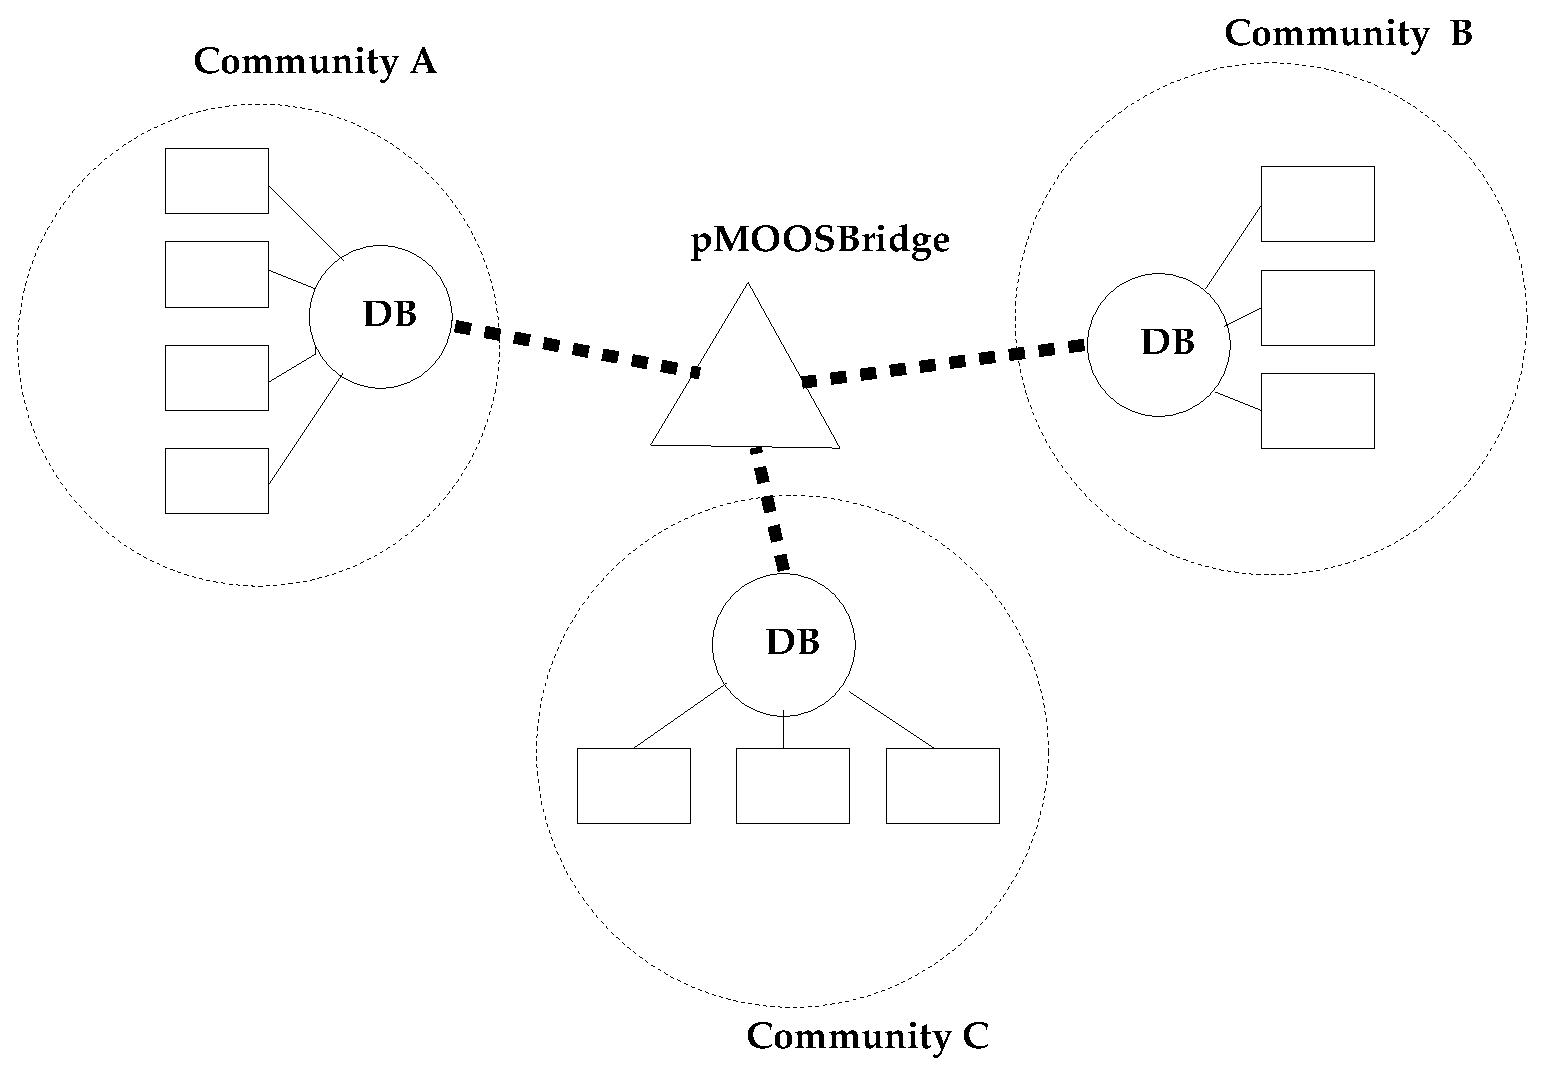
\epsfig{file = pMOOSBridge.eps , width = 0.6\linewidth}
\caption{A possible MOOSBridge
configuration.One instance of \code{pMOOSBridge} can ``talk'' to a limitless
number of communities. The configuration block specifies what
should be mapped or ``shared'' between communities and how it
should be done. The \code{SHARE} command specifies precisely what
variables should be shared between which communities.}\label{fig:MOOSBridge1}
\end{figure}
One instance of \code{pMOOSBridge} can ``talk'' to a limitless
number of communities. The configuration block specifies what
should be mapped or ``shared'' between communities and how it
should be done. The \code{SHARE} command specifies precisely what
variables should be shared between which communities and the
syntax is intuitive:\\

\code{SHARE= {\it{Comm@Host:Port[V1[,V2...]] $->$ Comm@Host:port
[V1,V2...]}}}\\

The triplet Comm@Host:Port is a description of a community ---  name and hostname/port pair. The community
description can be omitted on the l.h.s of the arrow in which case the mission-file-scope defaults are assumed (see the example below).
Each variable (``V'') on the l.h.s (source) community will be inserted into the community on the r.h.s.
If no variables names are specified on the r.h.s (destination) community the original names are used, otherwise
there is a one to one mapping between variable names on the l.h.s and new variable names (aliases) on the r.h.s. If however
there are more named shared variables than aliases, the variables for which a alias is not specified retain there original names.


For example\\
\begin{verbatim}
SHARE= VehA@nym.robots.ox.ac.uk:9000 [GPS_X]->VehB@kayak.mit.edu:9000 [GPS_X]
\end{verbatim}\\
Here the variable \code{GPS\_X} is shared between a community called ``VehA'' running from a \DB on the machine called
``nym.robots.ox.ac.uk' listening on port 9000 is being inserted into a community called ``VehB'' using a \DB running on the machine called
``VehB@kayak.mit.edu'' also listening on port 9000. In both communities the variable is called ``GPS\_X''. However when viewed with
something like \code{uMS} (see Section \ref{sec:MOOSScope} it can be seen that the \code{m\_sOrginatingCommunity} member of the \code{MOOSMsg}
carrying this data in the ``VehB'' commmunity will be ``VehA''.

\begin{verbatim}
SHARE= VehA@nym.robots.ox.ac.uk:9000 [GPS_X]->VehB@kayak.mit.edu:9000 [GPS_X_A]
\end{verbatim}
This is similar to the above example only \code{pMOOSBridge} will rename ``GPS\_X'' to ``GPS\_X\_A'' in the
destination community. The next example shows how the source address need not be specified. When omitted the source community is
taken to be the community on which \code{pMOOSBridge} is running at the time. This example also shows how destination variable names may be ommitted in
which case the original (source community) variable name is preserved.
\begin{verbatim}
SHARE= [GPS_X]->VehB@kayak.mit.edu:9000
\end{verbatim}
Finally more that one mapping can be specified in one line:
\begin{verbatim}
SHARE= [GPS_X,OVEN_TEMP]->VehB@kayak.mit.edu:9000 [GPS_X_A]
\end{verbatim}
here GPS\_X is being mapped and renamed to \code{GPS\_X\_A} in community ``VehB'' but the variable \code{OVEN\_TEMP} is simply being shared without renaming.
It is important to realise that sharing is not bidirectional. In this case a process notifying change in \code{GPS\_X\_A} in community ``VehB'' \emph{would not}
result in pMOOSBridge notifying the \DB in community ``VehA'' that ``GPS\_X'' has changed.


\begin{figure}[ht]
\centering \epsfig{file = pMOOSBridge2.eps , width =
0.6\linewidth} \caption{An alternative MOOSBridge Configuration
--- one bridge per community. This maybe preferable it is undesirable to have one process manage all
the sharing of data. However it offers no \emph{functional} advantage of the topology shown in Figure
\ref{fig:MOOSBridge1}.}\label{fig:MOOSBridge2}
\end{figure}



\newpage


\section{Manual Control - \code{iRemote}}\label{sec:iRemote}
%
\code{iRemote} was designed to be a control terminal for a
deployed vehicle. It is really nothing more than a long
\code{switch} statement based on characters input from the
keyboard. One of its many functions is to allow remote control of
the actuators of the vehicle. This is an invaluable asset for land
and sub-sea vehicles alike. The application is multithreaded. The
primary thread blocks on a read of keyboard input. When a
character is pressed some action is taken - for example publishing
a new value for \code{DESIREDTHRUST}. The fact that \code{iRemote}
can take control of a real vehicle presents a safety problem. What
if the human controller walks away or even worse the vehicle moves
out of communication range (eg a submarine dives) and the console
is not available? To prevent the last issued actuator command
being carried out {\it{ad-infinitum }} a secondary in thread
\code{iRemote} prompts the user to hit an acknowledge key (') at
least every 15 seconds. If the human driver does not respond the
all actuators are set to the zero position.\footnote{The actuation
driver  in iActuation will also shut down all motors if it does
not receive control commands for an extended period of time. In
the Bluefin vehicle the driver class within iActuation sends a
message to the Janitor processes which resets a watchdog on the
power management board - keeping the tail cone powered.}

\subsection{Summary of Functionality}
The following (not exhaustive) list describes some of the online
functionality that \code{iRemote} provides:

\begin{tabularx}{\linewidth}{l|c|X}
\textbf{Function} & \textbf{Key} & \textbf{Comment} \\ \hline

 Reload Mission File & \textsc{R} & Tells \code{pHelm} to
rebuild its
tasks \\
%
Restart Navigation & \textsc{V} & Tells \code{pNav} to reboot all
navigation filters
\\
%
Restart Logger  & \textsc{G} & Tells \code{pLogger} to begin
recording to a new set of log files \\
%
Begin Mission & \textsc{O} & Instructs \code{pHelm} to go online\\
%
Halt Mission & \textsc{O} or {\it{space}} & \code{pHelm} goes
offline and \code{iRemote} takes control immediately. \\
%
Navigation Summary & \textsc{*} & Prints a summary of salient
navigation information \\
%
Rudder Left/Right & \textsc{n},\textsc{m} & Steer control \\
%
Elevator Up/Down & \textsc{p},\textsc{l} & Pitch control \\
%
Thrust Up/Down & \textsc{a},\textsc{z} & Throttle control (+ shift
gives 100 percent) \\
%
Stop        & {\it{space}} & Immediate zero of all degrees of
freedom \\
%
Fetch DB       & \textsc{F} & Prints a summary of the contents of the entire \DB \\
%
CustomKey & $[0 \rightarrow 9]$ & The numeric keys can be made
(via \code{iRemote}s configuration block) to publish any named
variable with a specified value. In the example configuration
block below (Figure \ref{fig:iRemoteBlock}), pressing  key ``2''
will cause \code{iRemote} to write the variable
\code{JANITOR\_SWITCH} with the string value (quotes)
ACTUATION::OFF \\
%
CustomSummary & \textsc{+} & The configuration block allows a
custom summary to be built consisting of any variable names used
within the system. \code{iRemote} subscribes to this data and
prints its current value when requested.\\
%
{\New{CustomJournal}} & $[0 \rightarrow 9]$ & Similar to
{\it{CustomSummary}} but instead of keeping the most recently
published variable it keeps a history of values. Each Journal can
be  bound to a numeric key. In the example below pressing key
``6'' will show the past 10 values of \code{DESIRED\_RUDDER} with
every delta captured as the
capture time is 0.\\
\end{tabularx}

\begin{figure}[h]
\begin{lstlisting}[ ]{}
///////////////////////////////////////////////
// iRemote config block
ProcessConfig = iRemote
{
    CustomJournal = Name = DESIRED_RUDDER,Key =6, History = 10,Period = 0
    CustomSummary = DESIRED_THRUST
    CustomKey = 2 : JANITOR_SWITCH @ "ACTUATION:OFF"
}
\end{lstlisting}
\caption{A small configuration block for iRemote showing typical
usage of the \code{CustomX} commands}\label{fig:iRemoteBlock}
\end{figure}


\subsection{Informing the Pilot}
In most missions \code{iRemote} is the only interface the vehicle
pilot has with the vehicle. Clearly then a method is needed by
which {\em{important}} information can be sent to the
\code{iRemote} console from any process. The \code{CMOOSApp}
member function \code{MOOSDebugWrite} achieves this by issuing a
notification on a variable watched by \code{iRemote}. Such
messages are displayed on the iRemote console at run time along
with the process making the announcement. Note that this  name is
somewhat unfortunate as this function should not be used for
debugging - it is a run-time thing. It is frustrating to have a
cornucopia of messages flashing on the screen during a mission the
content of which is meaningless to the pilot. Typical uses of this
functionality would be a very occasional summary of navigation
status and system level warning messages - for example
notification of unexpected mission task  termination.

%

\section{Logging - \code{pLogger}}
The \code{pLogger} process is intended to record the activities of
a MOOS session. It can be configured to record a fraction of or
every publication of any number of MOOS variables. It is an
essential MOOS tool and is worth its weight in gold in terms of
post-mission analysis, data gathering and post-mission replay.

The configuration of \code{pLogger} is trivial and consists of
multiple lines with the following syntax:
\begin{center}
\code{Log} =  {\it{varname}} @ {\it{period}} $[NOSYNC]$
\end{center}
where {\it{varname}} is any MOOS variable name and {\it{period}}
is the minimum interval between log entries that will be recorded
for the given variable. For example if
{\it{varname}}=\code{INS\_YAW} and {\it{period}} = 0.2 then even
if the variable is published at 20Hz it will only be recorded at
5Hz. The optional \code{NOSYNC} flag indicates that this variable
should not be recorded in the synchronous logs (see section
\ref{sec:LogTypes})

\subsection{Log File Types}\label{sec:LogTypes}
The logger records data in two file formats - synchronous
(``slog'' extensions) and asynchronous (``alog'' extensions). Both
formats are ASCII text -- they can always be compressed later and
usability is more important than disk space. The two formats are
now discussed.

\subsubsection{Synchronous Log Files}
Synchronous logging makes a table of {\em{numerical}} data. Each
line in the file corresponds to a single time interval. Each
column of the table represents the broad evolution of a given
variable over time. The time between lines (and whether
synchronous logging is even required) is specified with the line
\begin{center}
\code{SyncLog}= {\it{true/false @ period}}
\end{center}
where {\it{period}} is the interval time.

If there has been no change in the numeric variable between
successive time steps then its value is written as \code{NaN}. It
is important to note that synchronous logs do not capture all that
happens - they sample it. Synchronous logs are designed to be used
to swiftly appraise the behaviour of a MOOS community by examining
numeric data in a tool such as Matlab or a spreadsheet. The
\code{MOOSData} Matlab script reads in these files and with a
single mouse click can display the time evolution of any logged
variable.


\subsubsection{Asynchronous Log Files}
Asynchronous logging is thorough. The mechanism is designed to be
able to record {\em{every}} delta to the MOOSDB. The use of the
period variable allows the mission designer to back off from this
ultimate limit and record variables at a maximum frequency. The
key properties of asynchronous can be enumerated as follows:
\begin{enumerate}
\item Records both string and numeric data
\item Records data in a list format - one notification per line
\item Entries only made when variable is written
\end{enumerate}
Asynchronous log files are designed to be used with a playback
tool (for example \code{uPlayback} or other purpose-built
executable). Although the handling of strings and numeric data
adds a slight overhead to such a program's complexity the utility
gain from being able to slow, stop and accelerate time during a
post-mission replay/reprocessing session is simply massive.


\subsubsection{Mission Backup}
Simply having the {\it{alog}} and {\it{slog}} files is not enough
to evaluate the mission. One also needs the things that
{\em{caused}} the data to be recorded, namely the *.moos Mission
file and the *.hoof file (if Task redirection was used). To this
end the \code{pLogger} process takes a copy of these files and
places them (name appended with a time stamp if desired) within
the logging directory. The files extensions are renamed to
{\it{*.\_moos}} and {\it{*.\_hoof}} respectively.



\section{Startup - \code{pAntler}}
The process \code{pAntler} is used to launch/create a MOOS
community. It is very simple and very useful. It reads from its
configuration block a list of process names that will constitute
the MOOS community. Each process to be launched is specfied with a
line with the syntax
\begin{center}
{\code{Run}} = {\it{procname}} [ @ {\code{NewConsole}} =
{\it{true/false}}] [$\sim$ \code{MOOSName}]
\end{center}
The optional console parameter specifies whether the named process
should be launched in a new  window (an xterm in Unix or
cmd-prompt in NT derived platforms). Each process launched is
passed the mission file name  as a command line argument. When the
processes have been launched \code{pAntler} waits for all of the
community to exit and then quits itself.

\subsubsection{Running Multiple Instances of a Process}

The optional \code{MOOSName} parameter allows MOOSProcesses to
connect to the \DB under a specified name. For example a vehicle
may have two GPS instruments onboard. Now by default \code{iGPS}
may register it existence with the \DB under the name ``iGPS''. By
using this syntax multiple instances of the executable \code{iGPS}
can be run but each connects to a the \DB using a different name.

\begin{center}
\code{Run = iGPS @ NewConsole = true $\sim$ iGPSA}\\
\code{Run = iGPS @ NewConsole = true $\sim$ iGPSB}\\
\end{center}

would launch two instances of \code{iGPS} registering under
``iGPSA'' and ``iGPSB'' respectively. Note there would need to be
\emph{two} GPS configuration blocks in the mission file -- one for
each and the processnames would be ``iGPSA'' and ``iGPSB''


\subsection{Usage}
\code{pAntler} provides a simple and compact way to start a MOOS
session. For example if the desired mission file is
{\it{Mission.moos}} then executing
\begin{center}
\code{pAntler Mission.moos}
\end{center}
will launch the required processes for the  mission. Of course a
sensibly designed mission will not actually start to do anything
until a human (via \code{iRemote}) has confirmed a good working
status of the processes involved (eg \code{pNav}) and actively
hands control over to the Helm.

\subsubsection{I/O Redirection - Deployment} As already mentioned,
frequently \code{iRemote}, displayed on a remote machine, will be
the only interface a mission pilot has to the MOOS community.  We
must ask the question -  ``where does all the IO from other
processes go to prevent I/O blocking?''. One answer to this is I/O
redirection and backgrounding MOOS processes - a simple task in
unix derived systems \footnote{some OS are good for development
others for running...}/

Running \code{pAntler} in the following fashion followed by a
manual start up of \code{iRemote} is the recommended way of
running MOOS in the field using a serial port login.

\begin{enumerate}
\item \code{pAntler} {\it{mission.moos}} $>$ ptyZ0 $>$ /dev/null \&
\item \code{iRemote} {\it{mission.moos}}
\end{enumerate}

This redirection of \code{iRemote} is encapsulated in the
\code{moosbg} script included with the MOOS installations. In the
case of an AUV the interface can only be reached  through in-air
wireless communications, which will clearly disappear when the
vehicle submerges but will gracefully re-connect when surfacing(
not so easy to do with a PPP or similar link).

\newpage
\part{Utilities}

\section{MOOS meets Matlab ---\code{iMatlab}}

Not everyone want to program in C++. Many folks are happy using
matlab as their research tool. Whilst not advising the use of
matlab to control a real vehicle, it seemed a useful to build an
application that allows matlab to join a MOOS community - if only
for listening in and rendering sensor data. The project
\code{iMatlab} allows that to happen. In essence it ``mex''s up
some central MOOS code so it can be called from inside matlab. The
\code{CMake} build system supported by current releases of MOOS
will build the project for Linux or Windows version of matlab.


\subsection{Configuration}

\code{iMatlab} allows Matlab programmers to access some of the
benefits of MOOS. It allows connection to the MOOSDB and access to
local serial ports. Configuration for the most part is done via a
*.moos file which is either the default iMatlab.moos found locally
or at a location specified at initialisation. Figure
\ref{fig:iMatlab} shows a typical configuration block for
\code{iMatlab}.

\begin{figure}[h]
\begin{lstlisting}[ ]{}
    ProcessConfig = iMatlab
    {
        AppTick     = 10
        CommsTick   = 10
        Port        = COM6
        BaudRate    = 4800
        Verbose     = false
        Streaming   = false
        MOOSComms = true
        SerialComms = false
        SERIAL_TIMEOUT = 10.0
        SUBSCRIBE = DB_TIME @ 0.0
    }
\end{lstlisting}
\caption{A typical configuration block for \code{iMatlab}
}\label{fig:iMatlab}
\end{figure}

Most of the fields are understandable by reading the MOOS
documentation. The application specific fields are:
\begin{description}
\item [MOOSComms]: ``true'' or ``false'' - do you want to connect to a
community?
%
\item [SerialComms]: ``true'' or ``false''  - do you want to use serial
ports ?
%
\item [SUBSCRIBE]: {\it{VariableName @ Period}} - one entry for each
variable you want to subscribe to and the maximum update rate you
are interested in . You can have many SUBSCRIBE lines.
\end{description}

Importantly always call \code{iMatlab('init')} first --- an error
message is printed if you forget. By default iMatlab looks to read
configuration data from iMatlab.moos. Alternatively you can use
\code{iMatlab('init','CONFIG\_FILE','XYZ.moos')} to read from the
file ``XYZ.moos''  You can specify a process name other than the
default ``iMatlab'' by passing the \code{MOOSName} parameter at
initialisation:
\code{iMatlab('init','MOOSNAME','MyName',.......)}.



\subsection{Usage}

If \code{MOOSComms} is ``true''  in the configuration file  then
MOOS Comms functionality is enabled.

\subsubsection{Publishing}
To send data use the following syntax
\code{iMatlab(\'MOOS\_MAIL\_TX\',VARNAME,VARVAL)} e.g
\newline \code{iMatlab('MOOS\_MAIL\_TX','A\_DATA\_VALUE',10)}
or\\
\code{iMatlab('MOOS\_MAIL\_TX','MY\_NAME','PMN')}\\

\subsubsection{Receiving Notifications}

To receive data use the syntax \code{ D =
iMatlab('MOOS\_MAIL\_RX')}.    This will return a structure array
describing the data that has arrived  (because of a subscription)
since the last call \code{'MOOS\_MAIL\_RX'} call . Each element of
$D$ will be a structure with the following fields given in Table
\ref{Tab:iMatlabMail}.

\begin{table}[h!]
\centering
\begin{tabularx}{\linewidth}{p{2.5in}|p{1in}|X}
\textbf{Field} &  \textbf{type} &\textbf{Description}\\
\hline
KEY                    & string & the name of the variable\\
TYPE                   & string & the type of the variable
('DBL'/'STR')\\
TIME                    &double & the time the data was valid\\
STR                    & string & the string value of the data if TYPE=='STR'\\
DBL                     &double & the double value of the data if TYPE=='DBL'\\
SRC                    & string & the name of the process that issued the data\\
ORIGINATING\_COMMUNITY &  string & the name of the community which
SRC belongs to\\\hline
\end{tabularx}
\label{Tab:iMatlabMail} \caption{The contents of a MOOS mail
structure in iMatlab} \normalsize
\end{table}




\subsubsection{Registering for Notifications}

This is done either through the configuration file using
\code{SUBSCRIBE=...} or by calling
\code{iMatlab('MOOS\_REGISTER',VarName,MinTime)} For example
calling \code{iMatlab('MOOS\_REGISTER','DESIRED\_RUDDER',0.0)}
will subscribe to \emph{every} change in \code{'DESIRED\_RUDDER'}
while calling
\code{iMatlab('MOOS\_REGISTER','DESIRED\_RUDDER',0.2)} will
subscribe in a way that means we'll only be told about changes in
'DESIRED\_RUDDER' every 0.2 seconds.


\subsection{Serial Ports}

If "SerialComms = true"  in the configuration file then serial
port functionality is enabled.

\subsubsection{Sending Data}

Call \code{iMatlab('SERIAL\_TX',Data)} where \code{Data} is a
string or a vector of type uint8.

\subsubsection{Reading Data}

To receive data on a serial port call \code{ D =
iMatlab('SERIAL\_RX',Data)}.If "Streaming=false" in the
configuration file then the function will block until a timeout
occurs or a telegram is received (ASCII, carriage return
terminated only in the release). If  \code{"Streaming  = true"}
the function returns immediately with a structure array containing
all the telegrams received since the last call. Each element of
$D$ is a structure described by Table \ref{Tab:iMatlabSerial}.


\begin{table}[h!]
\centering
\begin{tabularx}{\linewidth}{p{2.5in}|X}
\textbf{Field} &  \textbf{Description}\\\hline
            STR   & the data Rx'd\\
            TIME  & the time it was received\\
\hline
\end{tabularx}
\label{Tab:iMatlabSerial} \caption{The contents of the data
structure pertaining to received serial data in \code{iMatlab}}
\normalsize
\end{table}



\subsection{Other Functionality}

\subsubsection{Pausing}
Calling \code{ iMatlab('MOOS\_PAUSE',T)}  suspends the calling
thread (matlab itself in this case) for T seconds. This is pretty
useful for a non-busy wait in contrast to the CPU loading when
calling Matlab's own \code{pause} function.



\section{Replay -- \code{uPB}}
There is a FLTK-based, cross platform GUI application that can
load in {\it{alog}} files and replay them into a MOOS community as
though the originators of the data were really running and issuing
notifications. A typical use of this application is to ``fake''
the presence of sensor processes when reprocessing sensor data and
tuning navigation filters. Alternatively it can be used in pure
replay mode perhaps to render a movie of the recorded mission. The
GUI allows the selection of which processes are ``faked''. Only
data recorded from those applications will be replayed from the
log files.  There is a single class that encapsulates all the
replay functionality - \code{CMOOSPlayback}. The GUI simply hooks
into the methods exported by this class. The GUI is almost self
documenting - start it up and hold the mouse over various buttons.

\begin{figure}
\center \epsfig{file=uPB.eps,width = 0.5\linewidth} \caption{A
screen shot of \code{uPB} - a cross platform ``alog'' playback
tool}
\end{figure}

A client process can control the replay of MOOS messages by
writing to the \code{PLAYBACK\_CHOKE} variable add writing a valid
time in the numeric message field. The Playback executable will
not play more than a few seconds past this value before waiting
for a new value to be written. In this way  it is possible to
debug (halt inspect and compile-in-place etc) at source level a
client application using replayed data without having the playback
rush on ahead during periods of thought or code-stepping.


\section{Visual Debugging - \code{uMS}}\label{sec:MOOSScope}
The \code{uMS} is another GUI application. It allows a user to
place a stethoscope on the MOOS network and watch what variables
are being written, which processes are writing them and how often
this is happening. After starting up the scope and specifying the
host name and port number of the \DB the user is presented with a
list of all MOOS variable in the server and their current state.
Several times a second \code{uMS} calls into the DB and uses a
special/unusual (and intentionally undocumented) message that
requests that the server inform the client about {\em{all}}
variables currently stored along with their update statistics.
\code{uMS} is a central tool in the MOOS suite. It is cross
platform and should be used to spy on and present visual feedback
on any MOOS community.

\begin{figure}
\center \epsfig{file=uMS.eps,width = 0.9\linewidth} \caption{A
screen shot of \code{uMS} - a cross platform, multi-community
viewer.}
\end{figure}

\subsection{Improvements over \code{MOOSScope}}
\New{Improvement} \code{uMS} replaces the old , win32 only,
\code{MOOSScope}. As well as being cross platform It offers new
functionality:

\begin{itemize}
    \item Support for multiple communities via tabbed GUI.
    \item Memory of last settings (persistence)
    \item String expansion (click on long data strings and ballon
    appears.
    \item Show hide unassigned variables
    \item Show hide messages from specific processes
    (shift-leftclick on the process list)
    \item Poke the moos via ctrl-leftclick on a variable or empty
    cell.
\end{itemize}

\subsection{Poking the MOOS}
\code{uMS} has one other valuable use : poking the MOOS. It allows
a user to double click on a variable name and alter its value
(string or double) interactively. This is akin to changing memory
contents in a source code debugging session. The difference here
is that this action is a notification and all clients that are
registered for it receive a message in their mail box and act on
it accordingly. The utility of this functionality should not be
underestimated. For example, during the commissioning of a new
sensor (say a DVL) it may be unclear what the best configuration
parameters are. For example by having the managing process
subscribe for notifications on a \code{PARAMETERS} variable the
\code{uMS} can be used to rapidly explore the
performance/parameter space by simply poking new configuration
describing strings into the \code{PARAMETERS} variable.


\newpage
\section{Simulation --- \code{uMVS}}

\subsection{Simulation Mode}\label{Sec:SimMode}

There is is mission-file-scope variable \code{Simulator}. For
normal operation (i.e deployment of a real vehicle this will be
set to be true). However setting it to \code{false} enters MOOS
into a different mode - one of simulation.

The idea is that to gain confidence in new code its a good plan to
be able to do dry runs of all the code that will be expected to
govern the in-life operation of the vehicle. The Simulator flag in
conjunction with the behaviour of the instrument applications can
achieve this.

Setting the \code{simulator} flag to true causes the iProcesses
(instruments) to subscribe to one or more \code{SIM\_*} variables
like \code{SIM\_X},\code{SIM\_Y},\code{SIM\_DEPTH}. These
variables are published by a vehicle simulator (see Section
\ref{sec:uMVS}) and encapsulate the state of simulated vehicle.
The instruments then simulate their output using these values.

So to summarise : running in simulation mode means all the
instruments, navigation, Helm applications behave as normal,
passing and feeding off the same variables between each other.
However at the lowest level the instrument classes are not talking
to hardware via their serial ports etc but are subscribing to data
from a simulated world which they use to generate their
measurements.

For example iGPS normally talks to a GPS sensor via a serial port
and outputs \code{GPS\_X} etc. In simulation mode it also
subscribes to \code{SIM\_X} and \code{SIM\_Y} which it converts
internally (very simply, it turns out, by using the CMOOSVariable
class) into \code{GPS\_X}.


\begin{figure}[ht]
\centering 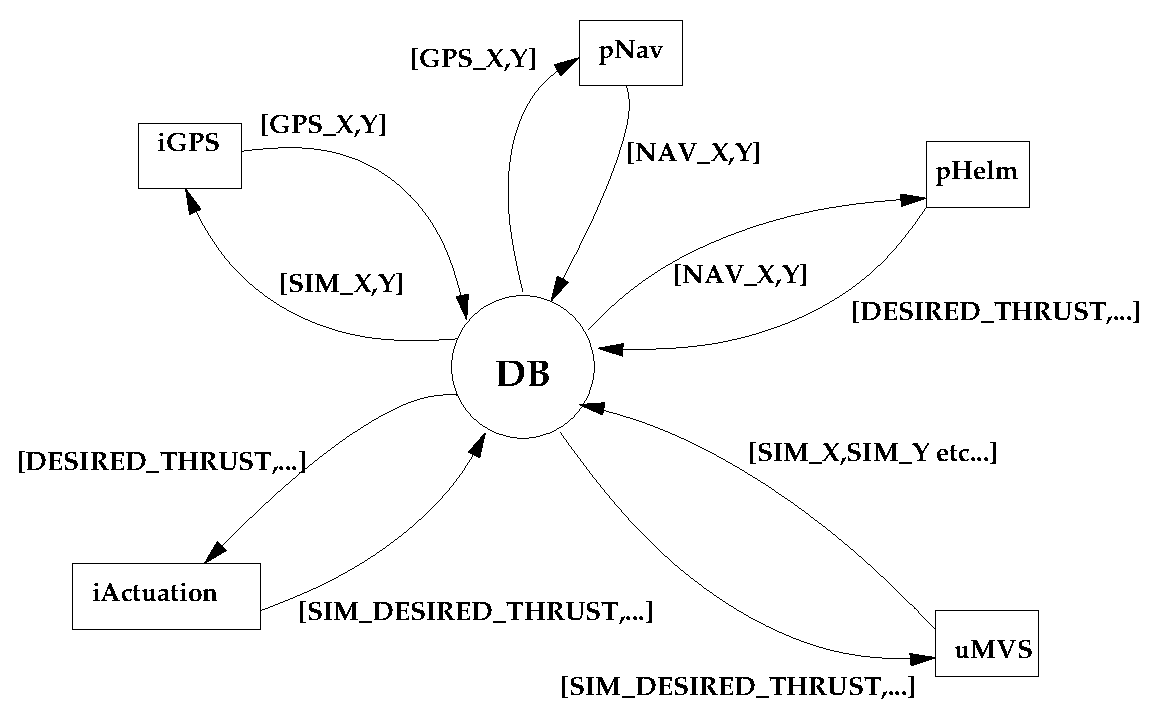
\epsfig{file = SimulationMode.eps , width =
0.8\linewidth} \caption{The variable subscription/publication
occurring  in simulation mode }\label{fig:SimulationMode}
\end{figure}

The final part of the story lies with \code{iActuation} - when in
simulation this process subscribes as usual to
\code{DESIRED\_RUDDER} etc but instead of sending bytes via a
serial port to a lump of hardware, it ``re-packages'' the commands
and bounces them back to the \DB as \code{SIM\_DESIRED\_RUDDER}
etc. It is these \code{SIM\_}-prefixed control  variables that are
subscribed to by the simulator and used to control the simulated
vehicle. This scenario is illustrated in Figure
\ref{fig:SimulationMode}. This shows how messages are bounced
around in the simulation mode - notice the additional \code{SIM\_}
prefixed subscriptions and publications made by \code{iGPS} and
\code{iActuation} respectively.

The details of the simulator is described in Section
\ref{sec:uMVS}.

\subsection{AUV and Acoustic Simulation  - \code{uMVS}}\label{sec:uMVS}
\code{uMVS} is a multi-vehicle AUV simulator. It is capable of
simulating any number of vehicles and acoustic ranging between
them and acoustic transponders. The vehicle simulation
incorporates a full 6D.O.F vehicle model replete with vehicle
dynamics, center of buoyancy/ center of gravity geometry, and
velocity dependent drag.

The acoustic simulation is also fairly smart. It simulates
acoustic packets propagating as spherical shells through the water
column. When they intersect with acoustic devices (either on
beacons or vehicles) the true time of intersection is calculated
by a refinement process. This design allows the real round trip to
be calculated when the vehicle is undertakes a trajectory that was
not known at the time the initial ``ping'' was launched.

A typical configuration block is given in \ref{fig:uMVSBlock}. The
syntax is simple --- consider the \code{ADD\_AUV} line in figure
\ref{fig:uMVSBlock}. The initial pose of the vehicle is specified
as an <X,Y,Z,Yaw> tuple. The AUV can also be named. The
\code{InputPrefix} and \code{OutputPrefix} terms are interesting.
They allow configuration of the names of the variables which are
used to control the actuators of the simulated vehicle and the
names of the variables used to describe the state of the vehicle.
As in reality, each vehicle is controlled by three actuator
settings : rudder,elevator and thrust. On a real vehicle these are
typically carried by the variables
\code{DESIRED\_THRUST},\code{DESIRED\_ELEVATOR} and
\code{DESIRED\_RUDDER}. Now say a particular simulated vehicle had
\code{InputPrefix = SIM\_}, \code{uMVS} would then subscribe to
\code{SIM\_DESIRED\_THRUST},\code{SIM\_DESIRED\_ELEVATOR} and
\code{SIM\_DESIRED\_RUDDER} and use these values as the control
parameters for the vehicle. Why might one like to do this? Well
see section \ref{Sec:SimMode}. An alternative use of the prefixes
is discussed in Section \ref{Sec:SimMinimal}.

\begin{figure}[h]
\begin{lstlisting}[ ]{}
ProcessConfig = uMVS
{
    //add an AUV, starting at Pose (X,Y,Z,Yaw), called AUV1.
    ADD_AUV=  pose=[4x1]{7,3,55,0},name = AUV1,InputPrefix=SIM_,OutputPrefix=SIM_
    ADD_TRANSPONDER=  name = B1, pose=[3x1]{0,0,0},Rx = CIF, Tx = Ch7,TAT = 0.125

    TideHeight = 60

    //a few variables for the simulator..
    LogFile = SimLog.txt
    InstantLogAcoustics = false

    //what is standard deviation of noise on
    //TOF measurements? 1ms = 1.5 meters
    TOFNoise = 0.00066
}

\end{lstlisting}
\caption{A small configuration block for \code{uMVS} showing a
typical configuration. This would be suitable for use with the
topology shown in Figure \ref{fig:SimulationMode}.
}\label{fig:uMVSBlock}
\end{figure}


\begin{figure}[h]
\begin{lstlisting}[ ]{}
ProcessConfig = uMVS
{
    ....
    ADD_AUV=  pose=[4x1]{7,3,55,0},name = AUV1,InputPrefix=,OutputPrefix=NAV_
    ....
}

\end{lstlisting}
\caption{Configuring the simulator to work for the scenario shown
in Figure \ref{fig:SimpleSim}. }\label{fig:SimpleuMVSBlock}
\end{figure}



\subsubsection{A more minimal simulation}\label{Sec:SimMinimal}

The ability to define the \code{InputPrefix} and
\code{OutputPrefix} terms for \code{uMVS} allows a more minimal
simulation to be constructed without using the global
\code{Simulation} flag discussed in Section \ref{Sec:SimMode}.
Infact one can eschew the need to use the instruments and
\code{iActuation} altogether. Why would anyone want to do this?
Well, the ``simulation mode'' of section \ref{Sec:SimMode} is
invaluable for gaining overall system/architecture confidence
however it can be inconvenient at times. For example if working on
the Helm or action planning process it may be inconvenient  to
have to launch the instrument processes and the Navigator at every
frequently during development. Figure \ref{fig:SimpleSim} shows an
alternative use of the simulator for exactly this case.  The
important configuration line (compared to \ref{fig:uMVSBlock}) is
shown in figure \ref{fig:SimpleuMVSBlock}. Note how the simulator
is told to publish \code{NAV\_*} data and subscribed to
\code{DESIRED\_THRUST},\code{DESIRED\_ELEVATOR},\code{DESIRED\_RUDDER}
by having an empty input prefix and \code{NAV\_} as an output
prefix. A typical topology using this set up is shown in Figure
\ref{fig:SimpleSim}.

\begin{figure}[ht]
\centering 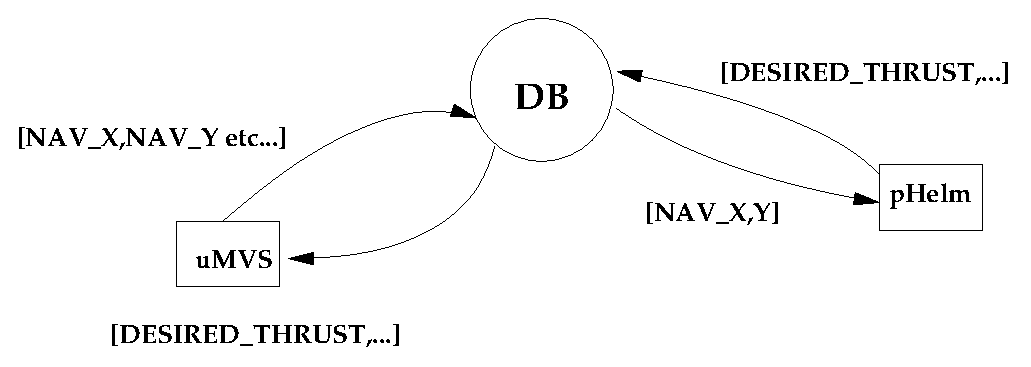
\epsfig{file = SimulationMode2.eps , width =
0.8\linewidth} \caption{A minimal simulation configuration for
example, Helm development. Here \code{uMVS} publishes vehicle
state as \code{NAV\_*} data and controls the internal simulated
vehicle by direct subscription to the standard Helm outputs.
}\label{fig:SimpleSim}
\end{figure}

\subsubsection{Logging}

\code{uMVS} can be configured (via the  \code{ LogFile} parameter)
to write a log file of the the simulation. This is a self
documenting file that records vehicle state and acoustic ranges
for perusal out of the MOOS environment.


\subsection{Multi-vehicle Simulation Scenarios}

So far we have considered the case of simulating a single vehicle
community (one community per vehicle). In the case there is one
mission file for the community, the simulator variable is set to
true and all process as run as though this were a real deployment
but behind the scenes the simulator is talking to the instruments
to fake reality. This was described in section \ref{Sec:SimMode}.

However what if it was desired to simulate (ie prepare for) and
experiment with multiple interacting vehicles, i.e lots of
communities how would this work? Several options are available to
the user here and they all involve the use of \code{pMOOSBridge}
which was described in section \ref{Sec:pMOOSBridge}.

One option is to run one simulator for each vehicle (each
simulator only running one vehicle) and use \code{pMOOSBridge} to
bridge whatever variables that need to be shared between
communities (it will most likely need to rename the variables
aswell). For example, consider Figure \ref{fig:MultiSim1}. Here a
possible two-vehicle simulation topology is shown. It is created
simply by linking two communities each with their own private
\code{uMVS} (here each in full simulation mode as described in
Section \ref{Sec:SimMode} but they could of course be in a reduced
form as described in Section \ref{Sec:SimMinimal}) with an
instance of \code{pMOOSBridge} described in Section
\ref{Sec:pMOOSBridge}.

\begin{figure}[ht]
\centering \epsfig{file = SimBridge0.eps , width = 0.8\linewidth}
\caption{A possible two-vehicle simulation created simply by
linking two communities each with a private \code{uMVS}(here each
in full simulation mode as described in Section \ref{Sec:SimMode}
but they could of course be in a reduced form as described in
Section \ref{Sec:SimMinimal}) with an instance of
\code{pMOOSBridge}.
 }\label{fig:MultiSim1}
\end{figure}


An alternative  approach would be to use the multi-vehicle
simulation capabilities of \code{uMVS} and adopt a topology
similar to Figure \ref{fig:MultiSim2}. Here each community has its
vehicle simulated in a common instance of \code{uMVS} which would
allow acoustic ranging between vehicles. Figure
\ref{fig:2AUVBlock} shows the possible configuration block for
\code{uMVS} in this scenario. Each vehicle community in Figure
\ref{fig:MultiSim2} runs its own instance of \code{pMOOSBridge} to
do the relevant data renaming between the ``simulating community''
and the rest of its own community. For example, with reference to
the configuration snippet in Figure \ref{fig:2AUVBlock} and the
topology of Figure \ref{fig:MultiSim2}, the bridge in ``Community
A'' would have to import \code{AUV\_A\_X} from the simulation
community and map it to \code{SIM\_X} while also export
\code{SIM\_DESIRED\_THRUST} as \code{AUV\_A\_DESIRED\_THRUST}
\footnote{And similarly for other relevant variables}.

\begin{figure}[ht]
\centering \epsfig{file = SimBridge.eps , width = 0.8\linewidth}
\caption{A possible two-vehicle simulation created simply by
linking two communities to a single ``simulation community'' via
private instances of \code{pMOOSBridge}. There is only one
\code{uMVS} running.
 }\label{fig:MultiSim2}
\end{figure}

\begin{figure}[h]
\begin{lstlisting}[ ]{}
ProcessConfig = uMVS {
    ....
    ADD_AUV=  pose=[4x1]{7,3,55,0},name = VehA,InputPrefix=AUV_A_,OutputPrefix=AUV_A_
    ADD_AUV=  pose=[4x1]{7,3,55,0},name = VehB,InputPrefix=AUV_A_,OutputPrefix=AUV_B_
    ....
}
\end{lstlisting}
\caption{Configuring the simulator to work for the scenario shown
in Figure \ref{fig:MultiSim2} with two vehicles. Note the values
of the input and output prefixes and the message renaming role
each \code{pMOOSBridge} has in Figure \ref{fig:MultiSim2} because
of them }\label{fig:2AUVBlock}
\end{figure}



\begin{figure}[ht]
\centering 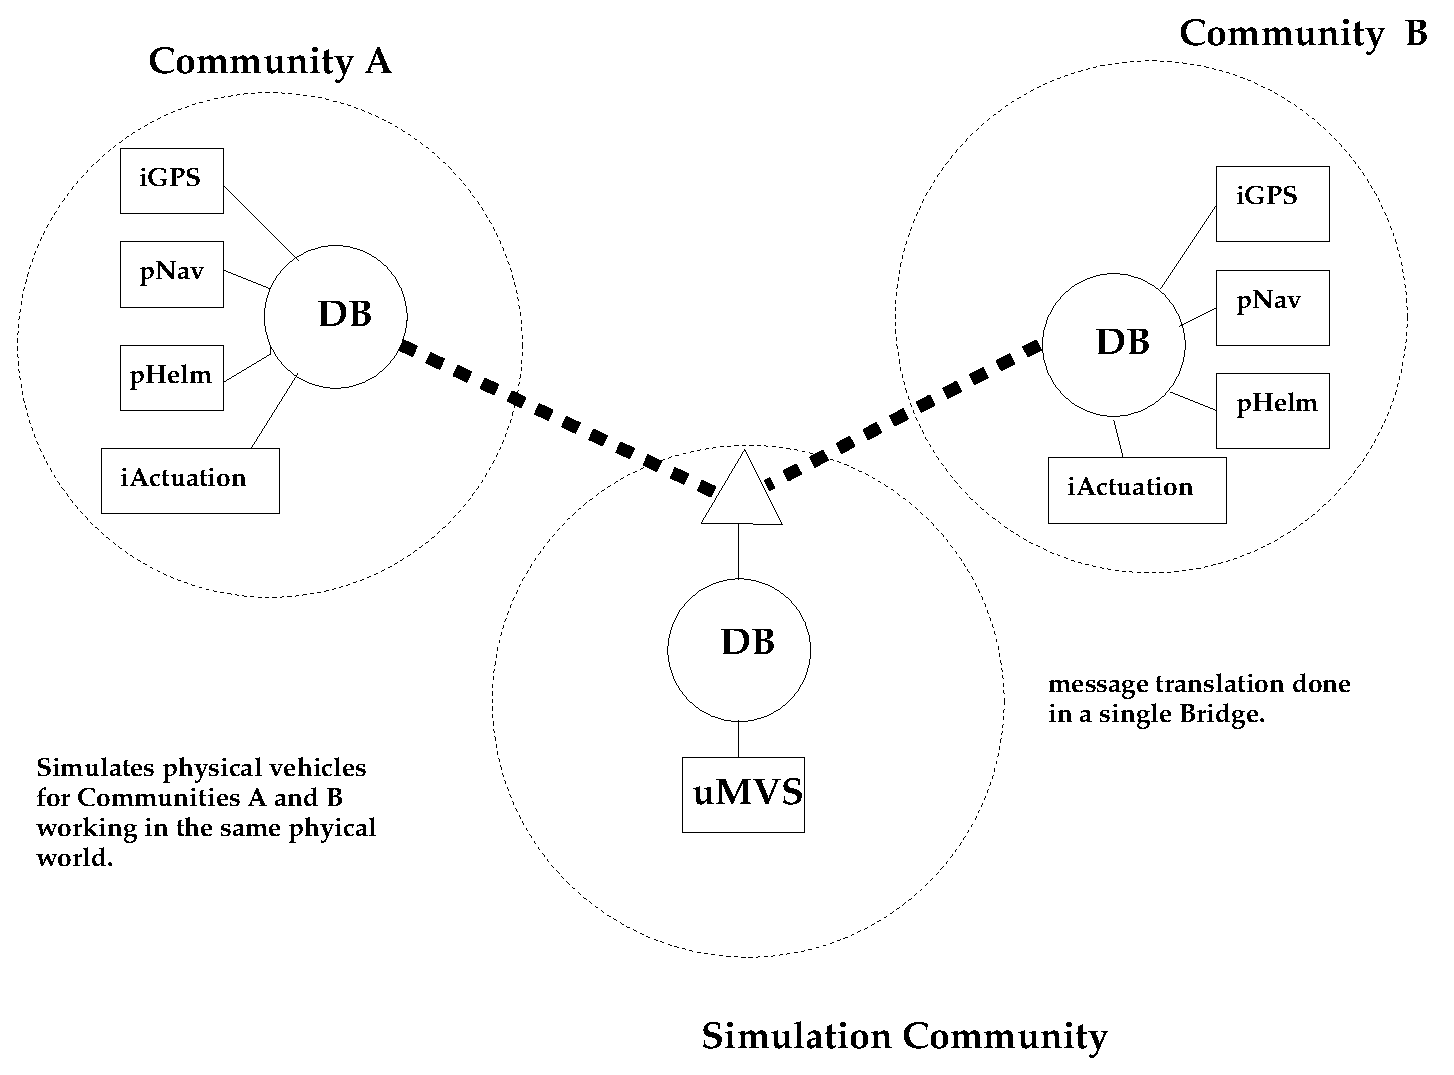
\epsfig{file = SimBridge2.eps , width = 0.8\linewidth}
\caption{A possible two-vehicle simulation created simply by
linking two communities to a single ``simulation community'' via a
{\emph{single}} instance of \code{pMOOSBridge}. Again, there is
only one \code{uMVS} running.
 }\label{fig:MultiSim3}
 \end{figure}

\begin{figure}[ht]
\centering 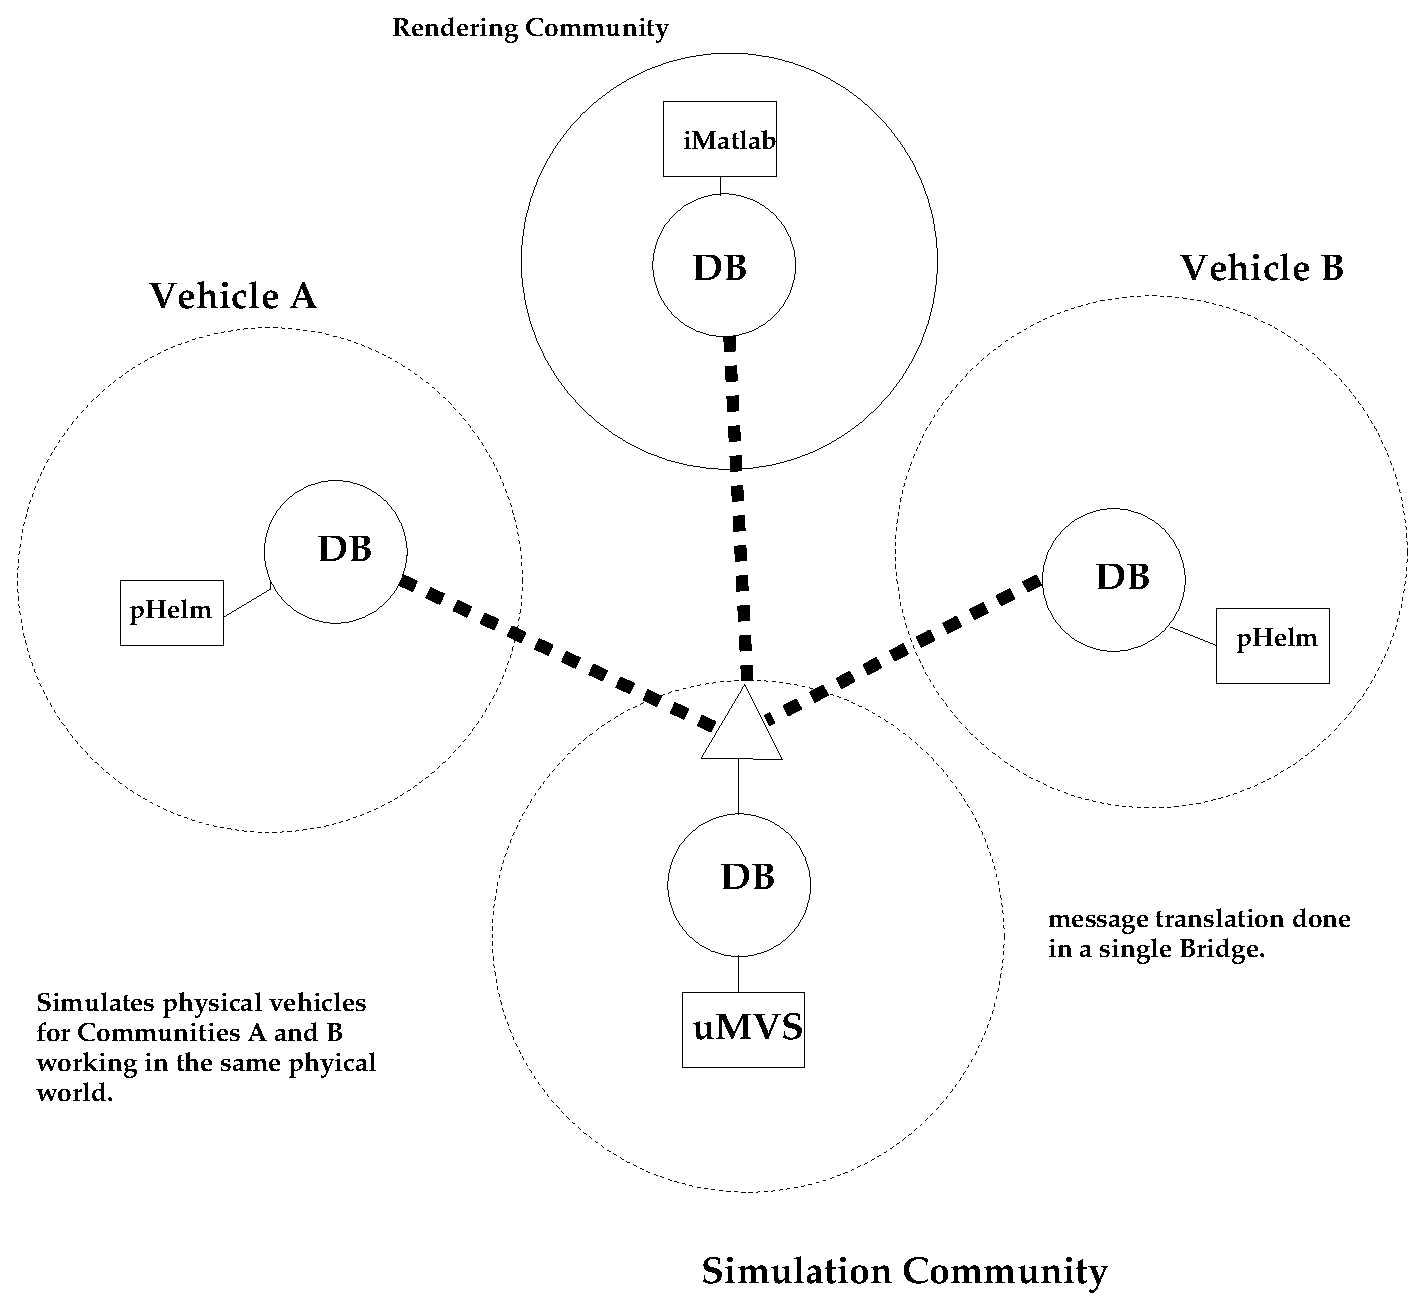
\epsfig{file = SimBridge3.eps , width = 0.8\linewidth}
\caption{Similar to \ref{fig:MultiSim3} where a two-vehicle
simulation is created simply by linking two communities to a
single ``simulation community'' via a {\emph{single}} instance of
\code{pMOOSBridge}. Again, there is only one \code{uMVS} running.
The difference between this topology and that shown in Figure
\ref{fig:MultiSim3} is the individual vehicle comunities are
{\emph{not}} running in simulation mode (described in Section
\ref{Sec:SimMode}). Instead, in this case, the single instance of
\code{pMOOSBridge} is renaming and routing data such that the need
for instruments and the navigator is avoided.
 }\label{fig:MultiSim4}
 \end{figure}
Finally, another two alternatives are presented in Figures
\ref{fig:MultiSim3} and \ref{fig:MultiSim4}. Here a single bridge
is used to do all the required data routing and name mapping for
both communities. In \ref{fig:MultiSim4}, a visualisation
community has been added which uses the \code{iMatlab} interface
to render the simulation in a ``fancy fashion''. Note that in this
case a minimal simulation is being run and so the Bridge will be
mapping, for example, \code{AUV\_A\_SIM\_X} on the simulation
community to \code{NAV\_X} on community \code{A} as well as
\code{AUV\_B\_SIM\_X} to \code{NAV\_X} on community \code{B}.

\subsubsection{Inter Vehicle Ranging}
The ``ADD\_AUV'' string can also specify how the vehicle acoustic system
responds to acoustic interrogation. By adding something of the form ``{\it{ResponderChannel = Ch3,TAT = 0.125}}'' to the ``ADD\_AUV'' string,
the vehicles will act like acoustic beacons (only they move) and respond to ``CIF'' pulses
from other vehicle transceivers on the channel specified with the declared turnaround-time.
If the ``ResponderChannel'' is not specified it will be assumed that inter-vehicle ranging
is not wanted and the vehicle's acoustic responders will be turned off.

\newpage
\part{Other Matters}
\section{Building MOOS}

All of the latest MOOS code found on
{\it{www.robots.ox.ac.uk/~pnewman}} is cross platform. Built into
the source tree is a cross platform build system that relies on
\code{CMake} - a thirdparty executable available from
{\it{www.cmake.org}} or the MOOS website.

\subsection{The Source Tree Shape}

\begin{figure}[ht]\label{fig:MOOSTree}
\centering 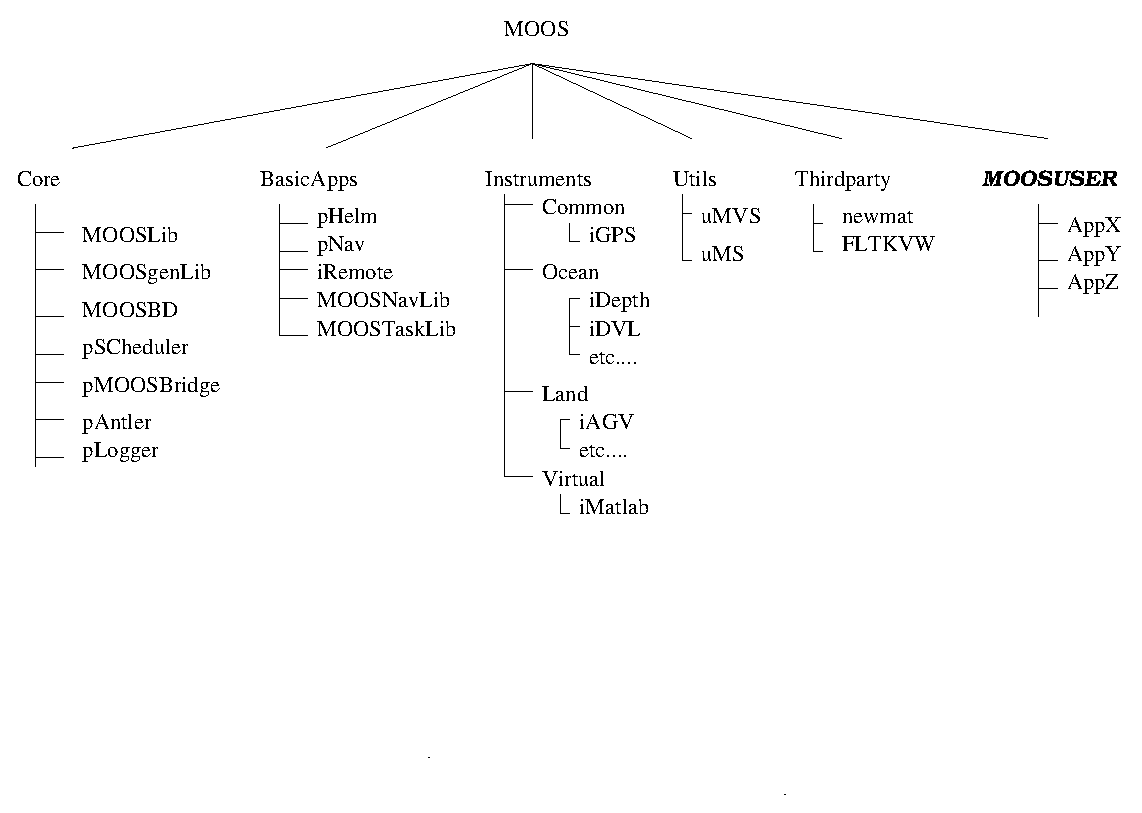
\epsfig{file = MOOSBuild.eps , width = \linewidth}
\caption{The MOOS source tree (as downloaded)}
\end{figure}

Figure \ref{fig:MOOSTree} shows the shape of the MOOS tree in
release packages. \footnote{you obviously don't have to stick with
this but it has some positives}. The ``core'' directory contains
code that has nothing per-se to do with robots. It is only
concerned with communications and logging communications. Of the
directories within ``core'' the most important three directories
are MOOSLib, MOOSGenLib and MOOSDB. These are the uber-core of
MOOS. The minimal conceivable build would be these three projects:
The base MOOS libraries and the MOOSDB server that binds processes
together.

The instruments subtree is pretty obvious - note it  includes
\code{iMatlab} which is peculiar instrument as it provides an
interface to Matlab not a device or human.

The \code{BasicApps} directory contains projects that are common
in mobile robotics apps --- \code{pNav} \code{pHelm} and
\code{iRemote}. \footnote{I would agree that there is a case to
put the latter in the instruments subfolder as it interfaces to a
``human instrument'' - but it seemed more robot centric rather
than sensor based - \it{sub-judice}}

The \code{Utils} directory is self explanatory and contains for
the most part cross platform GUIs and the a multi-vehicle AUV
simulator.

The Thirdparty directory contains cod that for the most past is
written by thirdparty authors. Newmat is linear algebra package
and FLTKVW is an extension to the FLTK functionality with a few
MOOS-Graphics additions.


\subsection{Cross platform Building using CMake}\label{Sec:CMake}

The use of \code{CMake} allows a code-author to describe in a high
level way what should be built in a project. The important point
from the is that it allows (via ``meta-make'' files called
\code{CMakeLists.txt} found in every directory) make files to be
written for unix and microsoft developer studio development alike.
This is a massive win in terms of cross platform development /
project management. \footnote{Of course if one only develops for
one OS it is hard to see the benefit.}

The instructions for building MOOS with \code{CMake} are as
follows:

\begin{enumerate}
\item  Download and install \code{CMake} for your platform (from
ww.cmake.org or the MOOS website)
%
\item ``cd'' into the MOOS root directory
%
\item Type \code{ccmake ./}  you should see
something like Figure \ref{fig:CMake1}.
\begin{figure}[ht]\label{fig:CMake1}
\centering 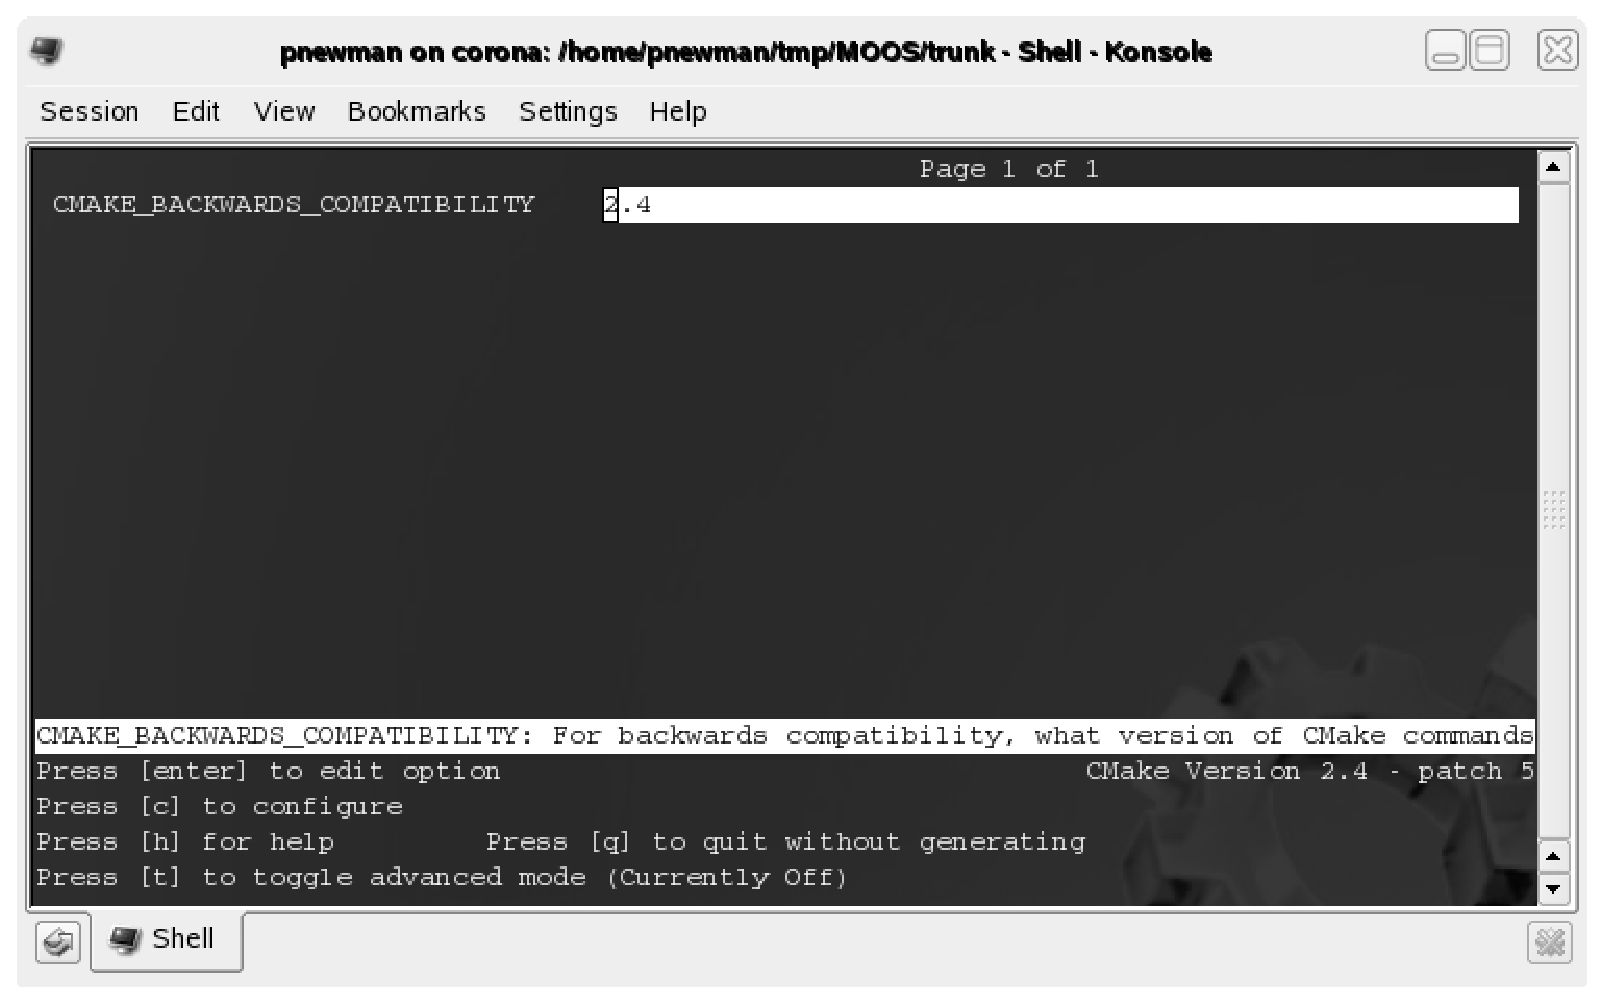
\epsfig{file = CMake1.eps , width =  0.8\linewidth}
\caption{The initial CMake Screen - Win32 platforms have a
gui-dialog rather than an ncurses interface}
\end{figure}
%
\item press "c" to configure - the screen should look like
something like Figure \ref{fig:CMake2}.
\begin{figure}[ht]\label{fig:CMake2}
\centering 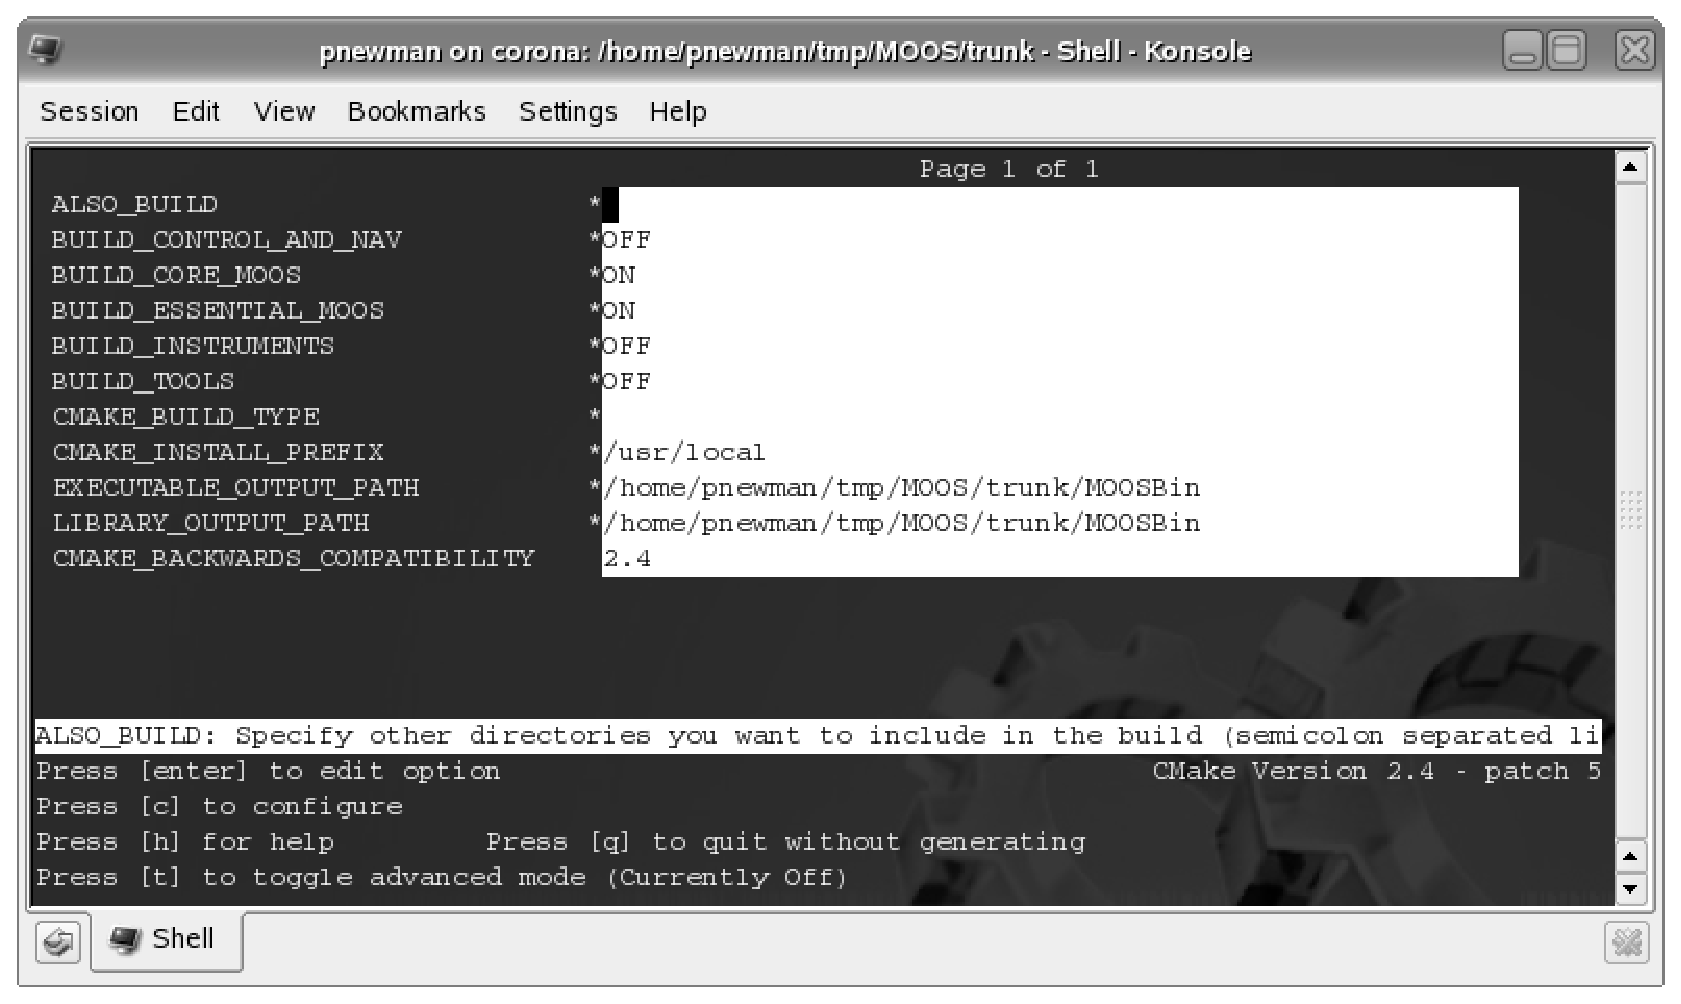
\epsfig{file = CMake2.eps , width = 0.8\linewidth}
\caption{The initial CMake Screen after an initial configure -
note no option to generate makes files is present as yet. Build
directories and build options (ie what to build and what not) can
be selected at this stage. }
\end{figure}
*
\item press "c" to configure once more. the screen should now look
something like  Figure \ref{fig:CMake3}.
\begin{figure}[ht]\label{fig:CMake3}
\centering 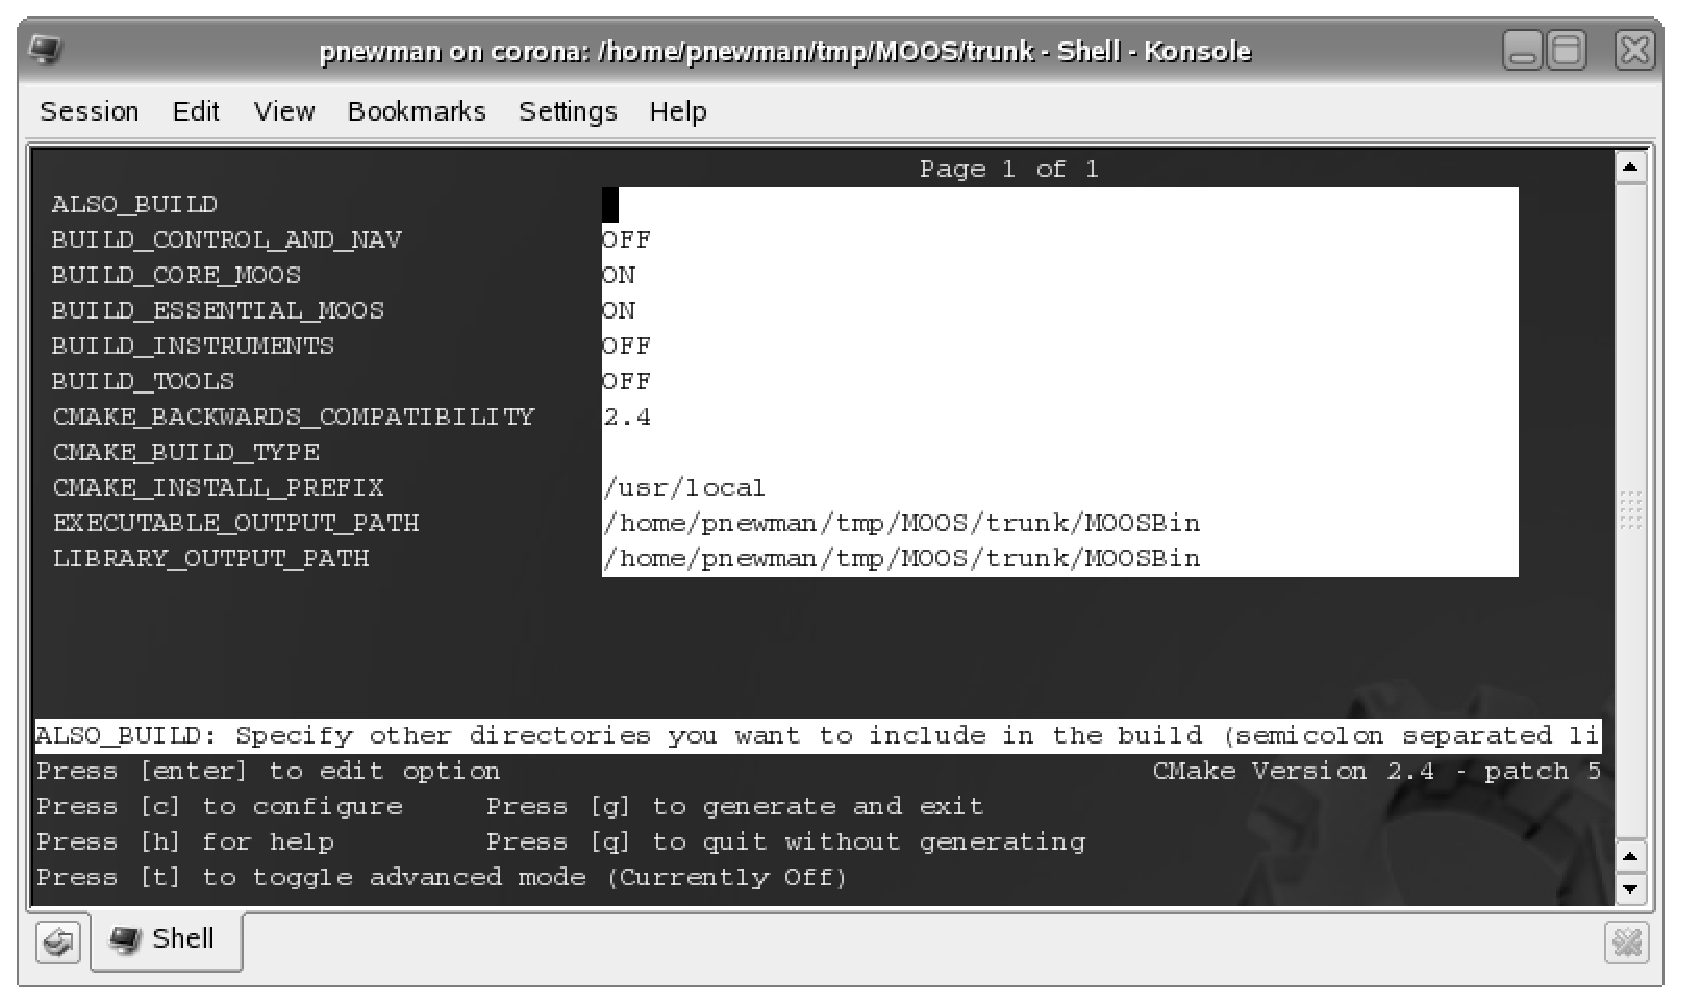
\epsfig{file = CMake3.eps , width = 0.8\linewidth}
\caption{The final CMake Screen before generating the build files
(``.dsp'' or Makefile --- depending on platform). Please note
``Configure'' may have been selected several times before this
final option is presented. }
\end{figure}
%
\item Notice an option "g" has appeared saying we are good to
go....Press "g" to generate the MOOS make files. If you have
followed the above steps CMake will exit and you'll see (along
with one or two other CMake generated files) a master Makefile in
the root directory. Typing make at the prompt will now cause the
MOOS core to be built. Check it does!
\end{enumerate}


By toggling the relevant fields in the ccmake curses-GUI you can
turn on/off Makefile generation for different part of the project.
Pressing "c" to configure then parses the newly included
CMakeLists.txt files and may present some new option for you to
select. Things should work simply by accepting the default values.

Note, the Utils directory includes massively useful GUI
applications which link against FLTK. You are expected to have the
library and include files in your system path (this should have
been done for you using the configure, make,make install paradigm
when building the FLTK library) Part III Adding your own projects
to the build tree

By entering a suitable directory or symbolic link in the
\code{ALSO\_BUILD} field causes CMake to recurse into tat
directory when creating make files. This way developers can
include their own projects in the build paradigm. For example, the
Oxford Mobile Robotics group has a directory called OXMOOS which
lives in a directory in MOOS (just like Core or Utils does).
Typing OXMOOS in the \code{ALSO\_BUILD} field causes CMake to
recurse into the OXMOOS directory and follow the instructions in
the CMakeLists.txt file therein (which causes it to recurse
further down into each of our individual application projects).
The advantage of this is it inherits all the build flags, library
settings of the parent MOOS project and so things like the library
paths (MOOSBin in the example above) are automatically passed to
the compiler.\\ \vspace{1cm}\\ \textbf{By default binaries and
libraries are placed in MOOS/MOOSBin} - this of course can be
changed simply by typing in your preferred destination during the
build system set up using CMake \footnote{Devstudio users will
find the binaries in debug/release/releasewithdebug directories
within MOOSBin depending on the active project configuration
selected in the IDE.} See Figure \ref{fig:CMake2}.


\subsection{Incorporating a Private Codebase/Subtree}

It is recommended to place a private subtree where the
``MOOSUSER'' label is in Figure \ref{fig:MOOSTree}. For example
the author has a private source tree called ``OXMOOS'' which can
normally be found in this location - a sibling of ``BasicApps''
and ``Core'' etc. The code{CMake} (See section \ref{Sec:CMake})
insfrastucture can be directed to descend into this subtree by
specifying the name of the subtree in the {\it{``ALSO\_BUILD''}}
field of the \code{CMake} configuration pages.


\subsection{I insist on my own Makefiles...}

Some MOOS users may not wish to use the CMake infrastructure  (a
CMakeLists.txt file in each directory) or tree provided in the
releases
--- preferring instead to use old trusted make files they have
written themselves for whatever platform they wish to
develop/deploy on. This of course will work --- the source in no
way depends upon the build system. The following tips maybe
useful:

\begin{itemize}
    \item The CMakeLists.txt files are a good way to see what
    needs to be built. The sources are listed and so are the
    linking dependencies.
    \item Don't assume all files in a directory should be compiled
    into an executable. Although this is generally true there are
    some applications that have OS dependent source-sets.
    \item To compile a MOOS applications it will need to have
    {\it{MOOS/Core}}in the include path and link against
    {\it{MOOSGen.a}} and {\it{MOOS.a}}. Where these are built depends on
    your own make files.
\end{itemize}

\newpage
\part{Summary and Further Work}

This paper provides a discussion of the MOOS software. It is
however, by no means exhaustive. Although the architecture of the
core communications are completely described many of the details
of the higher level processes building on this architecture have
been omitted. In some ways this is in the spirit of the MOOS -
knowledge of the innards of individual processes can be
administered on a ``need to know basis''. What is important is the
interactions between processes. In a similar vein the details of
of the workings navigation filters have also been omitted although
their broad functionality is described.

It is hoped that MOOS can provide a flexible research tool for
some time to come. It is an evolving project and under continual
improvement and expansion.

Most of all it should be fun to use -  despite its ridiculous
name.

\Ignore{
\section{StillToDo }

\begin{itemize}
  \item scheduler
  \item uMVS
  \item iMatlab
  \item SourceTree and Building
\end{itemize}
}






















%%%%%%%%%%%%%%%%%%%%%%%%%%%%%%%%%%%%%%%%%%%%%%%%%%%%%%%%%%%%%%%%%%%%%%%%%%%%%%%%%%%%%%%%%%%%%%%%%%%%
\newpage
\appendix
\section*{Appendix A - Skeleton Code}\label{app:A}

\begin{figure}[h!]
\begin{lstlisting}[]{}
#include "MOOSLib.h"
#include "MOOSGenLib.h"
#include "Skeleton.h"
int main(int argc ,char * argv[]) {
    // set default mission file
    char * sMissionFile="Mission.moos";

    if(argc>1)
    {
        sMissionFile = argv[1];
    }

    //make your application
    CSkeleton TheSkeleton;

    //run it//
    TheExample.Run("Skeleton",sMissionFile);

    return 0;
}
\end{lstlisting}
\caption{source code for a very minimal application that runs a
\code{CMOOSApp} derived object called \code{TheSkeleton} of type
\code{CSkeleton}.}
\end{figure}

\begin{figure}
\begin{lstlisting}[]{}
class CSkeleton : public CMOOSApp
{
 protected:
    //these are the virtual functions to overide
    bool OnNewMail(MOOSMSG_LIST &NewMail);
    bool Iterate();
    bool OnConnectToServer();
    bool OnStartUp();
};
\end{lstlisting}
\caption{source code for the declaration of the example
\code{CSkeleton} class}
\end{figure}
%
\begin{figure}

\begin{lstlisting}[ ]{}
#include "Skeleton.h"

bool CSkeleton::OnNewMail(MOOSMSG_LIST &NewMail)
{
    //parse mail here
    return true;
}

bool CSkeleton::OnConnectToServer()
{
    //register for variables here....
    return true;
}

bool CSkeleton::Iterate()
{
    //do standard work here
    return true;
}

bool CSkeleton::OnStartUp()
{
    //do start up things here...
    //for example read from mission file...
    return true;
}
\end{lstlisting} \caption{source code for the \code{CSkeleton}
\code{MOOSApp} derived class}
\end{figure}
\newpage
\section*{Appendix B - Navigation Configuration}
\begin{lstlisting}[ ]{}
/////////////////////////////////////////////
// pNav control block
ProcessConfig = pNav {

    ///////////////////////////////////////////
    //      routing priority stack
    ///////////////////////////////////////////
    X           = GPS @ 2.0,EKF @ 2.0 ,LSQ @ 5.0,
    Y           = GPS @ 2.0,EKF @ 2.0 ,LSQ @ 5.0,
    Z           = EKF @ 2.0 ,LSQ @ 5.0,
    Depth       = EKF @ 2.0 ,LSQ @ 5.0, DEPTH @ 1.0
    Altitude    = RANGE @ 1.0
    Yaw         = EKF @ 2.0 ,LSQ @ 5.0, INS @ 1.0
    Pitch       = INS
    Speed       = EKF

    ALWAYS_READ = INS_YAW,PARA_DEPTH,LBL_TOF,GPS_X,
                  GPS_Y,DVL_BODY_VEL_Y,DVL_BODY_VEL_X,DESIRED_THRUST

    /////////////////////
    //  FILTER CONTROL:
    /////////////////////

    //what filters to use......
    UseLSQ      = true
    UseEKF      = true
    LSQTimeOut  = 180

    MaxLSQEKFDeviation = 20
    MaxEKFPositionUncertainty = 30

    //how to log nav if required (development tool)
    NAV_LOG = true
    NAV_LOG_PATH = C:\codescratch\MOOSLOG\
    NAV_LOG_TIMESTAMP = false


    SV = 1500.0

    ///////////////////////////////
    // static observations
    // format is  [Value] @ [uncertainty]
    ///////////////////////////////

    FixedTide       = 0 @ 0.1

    ////////////////////////////////
    // map sensor outputs to sensors within filters
    // specifying geometry.....
    // Syntax is as follows
    // SensorType       =Source -> SensorName @ Location ~ Sensor Std
    //////////////////////////////

    SENSOR_XY       =   iGPS    ->  TheGPS    @ 0,0,0 ~ 0.3
    SENSOR_LBL      =   iLBL    ->  TheAvtrak @ 0,0,0 ~ 0.009
    SENSOR_ORIENTATION  =   iINS    ->  TheINS    @ 0,0,0 ~ 0.01
    SENSOR_DEPTH        =   iDepth  ->  TheDepth  @ 0,0,0 ~ 0.1
    SENSOR_BODY_VEL     =   iDVL  ->    TheDVL    @ 0,0,0 ~ 0.05


    ///////////////////////////////
    // Least Square filter set up
    LSQ_REJECTION = TheAvtrak[1] :  History = 6 ,FAIL = 0.005
    LSQ_REJECTION = TheAvtrak[2] :  History = 6 ,FAIL = 0.005
    //etc...
    //etc...

    ///////////////////////////////
    // Extended Kalman Filter set up

    EKF_LAG =3.0
    EKF_TIDE = 00

    //how fast/mobile is the vehicle?
    // 1=slow
    // 10 =fast
    EKF_XY_DYNAMICS = 0.1
    EKF_Z_DYNAMICS = 0.1
    EKF_YAW_DYNAMICS = 0.1
    EKF_VEHICLE_TYPE = MOBILE

    //initial uncertainty
    EKF_SIGMA_XX = 20.5
    EKF_SIGMA_YY = 20.5
    EKF_SIGMA_ZZ = 1
    EKF_SIGMA_HH = 180
    EKF_SIGMA_TIDE = 0.1

    //initial state
    EKF_X = 0
    EKF_Y = 0
    EKF_Z = 0
    EKF_H = 0
}
\end{lstlisting}
%\end{figure*}

\section*{Appendix C - Coding Style Guide}
This is the recommended coding style for c++ in MOOS. The author
has tried to follow such rules throughout - of course there will
be occasional slips and these should be corrected where found -
its all about entropy\footnote{Thanks to Greg Walker for this
list}. The author urges future ``MOOSies'' to use the same style.
It is not so much about one style being better than another but
keeping things unified  and having the same flavor whenever
possible.
\begin{itemize}
    \item  Use Hungarian notation prefixes for variables"
    \begin{itemize}
            \item doubles prefixed by "df" eg "dfMyLocalVal"
            \item ints prefixed by "n"
            \item strings prefixed by "s"
            \item member variables begin with "m\_" eg "m\_dfMyMemberVal"
    \end{itemize}
    \item  Variables should be long enough to be meaningful.  Where they are multi word use capital to denote first letter of each word.  e.g. m\_dfTurnAroundTime.
    \item  Use capital letters to identify defined constants (or the equivalent thereof)
    \item  Indent / tab stops in steps of 4
    \item  Opening and closing brackets at same tab stop as outer, enclosed lines to be indented.
    \item Minimize scope of local variables.
    \item Do not re-use a single local variable to express different concepts at different points in a routine.  There is a risk that somebody doesn't notice that when he comes to modify code at a later date.
    \item Be liberal in use of white space to separate logical steps - for clarity.
    \item Source text should not overrun 100 characters to a line.  You should be able to get that across a portrait style A4 paper page if you want to print it out.
    \item Keep to simple expressions in a statement.  It will be easier to understand later.
    \item Restrict the executable code of a procedure to about an A4 page.  If it stretches much beyond that you can probably find a block of code that expresses an identifiable concept to remove to a separate procedure.
    \item Avoid the use of multiple inheritance and friend classes.
    \item Never sit in an un-blocked loop waiting for an externally controlled condition to be met.  It eats up processor time with no benefit.
    \item Avoid use of explicit numeric values in code.  Assign symbolic name to the number so that the definition appears in one place only.
    \item Avoid "copy and paste" of anything more than tiny code fragments.  It's an indication that a common procedure can be created which will service multiple needs.  If there's less code in the application, there's less to go wrong.  If it needs a fix then one fix solves all associated problems - you don't have to seek out the other similar code which probably has the same fault.
    \item Where procedure calls have lots of parameters, don't be afraid to assign a line to each parameter - but do put the opening bracket in the same text column as the closing bracket.
    \item TRACE statements should start with class::method identifier, and end with a newline.  That makes it easy to find the source code that invoked the debug output.  e.g. TRACE("CMyClass::DoIt - That's done it $\backslash$ n");
\end{itemize}

\section*{Appendix D - Known Bugs and Inadequacies}
The following is an incomplete list of the known issues with MOOS
as of December 2002.

\begin{itemize}
\item Navigation filters do not take roll and pitch into account
when processing DVL data - easy to fix as all sensor data is
transformed into to a horizontal, rotated frame for processing.
\item In Windows \code{iRemote}sometimes does not quit when told
to. Strangely it does remove itself from the process table.
\item The dynamic controllers do not take in rate information but
rather infer it themselves which is a noise prone process and
incurs a phase lag - easy to fix.
\end{itemize}

\end{document}
